\documentclass[%draft,
    10pt,
    headinclude, footexclude,
    % twoside, % this produces strange margins!
    openright, % for new chapters
    notitlepage,
    cleardoubleempty,
    headsepline,
    pointlessnumbers,
    bibtotoc, idxtotoc,
    ]{scrbook}

% iPad Air 2 resolution: 1536 x 2048
% 1.3333 ratio (4:3)
% LeeSeshia is 15,73 ? 20,96 cm, ratio 1.332
%\setlength{\paperwidth}{15.73cm} \setlength{\paperheight}{20.96cm}
\setlength{\paperwidth}{15.72cm} \setlength{\paperheight}{20.95cm}
%\typearea{calc} % without BCOR results to a DIV of 8 for 11pt
\typearea[1cm]{18} % TODO: check if 1 cm is the correct number

\usepackage{scrlayer-scrpage}
\setkomafont{pagehead}{\scshape\small}
\setkomafont{pagenumber}{\scshape\small}


\newif\ifbook
\booktrue % comment out for the eBook version

\ifbook
\else
\cfoot{\hyperlink{contents}{Contents}}
\fi




\usepackage{pslatex} % -- times instead of computer modern, especially for the plain article class
\usepackage[colorlinks=true,bookmarks=false]{hyperref}
\usepackage{booktabs}
\usepackage{graphicx}
\usepackage{xcolor}
\usepackage{multirow}
\usepackage{cite}
%\usepackage{flushend} % even out the last page, but use only at the end when there is a bibliography
\usepackage{dirtree}
\usepackage{pdfpages}
% For alignment on tables
\usepackage{dcolumn}
\newcommand{\cc}[1]{\multicolumn{1}{c}{#1}}

\newcommand{\code}[1]{{\small{\texttt{#1}}}}
\newcommand{\codefoot}[1]{{\footnotesize{\texttt{#1}}}}

% fatter TT font
\renewcommand*\ttdefault{txtt}
% another TT, suggested by Alex
% \usepackage{inconsolata}
% \usepackage[T1]{fontenc} % needed as well?

\usepackage[procnames]{listings}


\ifbook
\hypersetup{
  linkcolor  = black,
  citecolor  = black,
  urlcolor   = black,
  colorlinks = black,
  bookmarks=false,
}
\else
\hypersetup{
  linkcolor  = blue,
  citecolor  = blue,
  urlcolor   = blue,
  colorlinks = true,
  bookmarks=true,
}
\fi

% not really used
\newenvironment{comment}
{ \vspace{-0.1in}
  \begin{quotation}
  \noindent
  \small \em
  \rule{\linewidth}{0.5pt}\\
}
{
  \\
  \rule{\linewidth}{0.5pt}
  \end{quotation}
}

\newcommand{\scale}{0.7}

% shared in slides and book

\lstdefinelanguage{chisel}{
  morekeywords={abstract,case,catch,class,def,%
    do,else,extends,false,final,finally,%
    for,if,implicit,import,match,mixin,%
    new,null,object,override,package,%
    private,protected,requires,return,sealed,%
    super,this,throw,trait,true,try,%
    type,val,var,while,with,yield},
  otherkeywords={=>,<-,<\%,<:,>:,\#,@},
  sensitive=true,
  morecomment=[l]{//},
  morecomment=[n]{/*}{*/},
  morestring=[b]",
  morestring=[b]',
  morestring=[b]"""
}

\usepackage{color}
\definecolor{dkgreen}{rgb}{0,0.6,0}
\definecolor{gray}{rgb}{0.5,0.5,0.5}
\definecolor{mauve}{rgb}{0.58,0,0.82}

% Default settings for code listings
\ifbook
\lstset{%frame=lines,
  language=chisel,
  aboveskip=3mm,
  belowskip=3mm,
  showstringspaces=false,
  columns=fixed, % basewidth=\mybasewidth,
  basicstyle={\small\ttfamily},
  numbers=none,
  numberstyle=\footnotesize,
  % identifierstyle=\color{red},
  breaklines=true,
  breakatwhitespace=true,
  procnamekeys={def, val, var, class, trait, object, extends},
  % procnamestyle=\ttfamily,
  tabsize=2,
  float
}
\else
\lstset{%frame=lines,
  language=chisel,
  aboveskip=3mm,
  belowskip=3mm,
  showstringspaces=false,
  columns=fixed, % basewidth=\mybasewidth,
  basicstyle={\small\ttfamily},
  numbers=none,
  numberstyle=\footnotesize\color{gray},
  % identifierstyle=\color{red},
  keywordstyle=\color{blue},
  commentstyle=\color{dkgreen},
  stringstyle=\color{mauve},
  breaklines=true,
  breakatwhitespace=true,
  procnamekeys={def, val, var, class, trait, object, extends},
  procnamestyle=\ttfamily\color{red},
  tabsize=2,
  float
}
\fi

\lstnewenvironment{chisel}[1][]
{\lstset{language=chisel,#1}}
{}

\newcommand{\shortlist}[1]{{\lstinputlisting[nolol]{#1}}}

\newcommand{\longlist}[3]{{\lstinputlisting[float, caption={#2}, label={#3}, frame=tb, captionpos=b]{#1}}}

\newcommand{\verylonglist}[3]{{\lstinputlisting[caption={#2}, label={#3}, frame=tb, captionpos=b]{#1}}}


\newcommand{\todo}[1]{{\emph{TODO: #1}}}
\newcommand{\martin}[1]{{\color{blue} Martin: #1}}
\newcommand{\myref}[2]{\href{#1}{#2}}

\ifbook
\renewcommand{\myref}[2]{{#2}{\footnote{\url{#1}}}}
\fi

% uncomment following for final submission
\renewcommand{\todo}[1]{}
\renewcommand{\martin}[1]{}

\begin{document}


\ifbook
\else
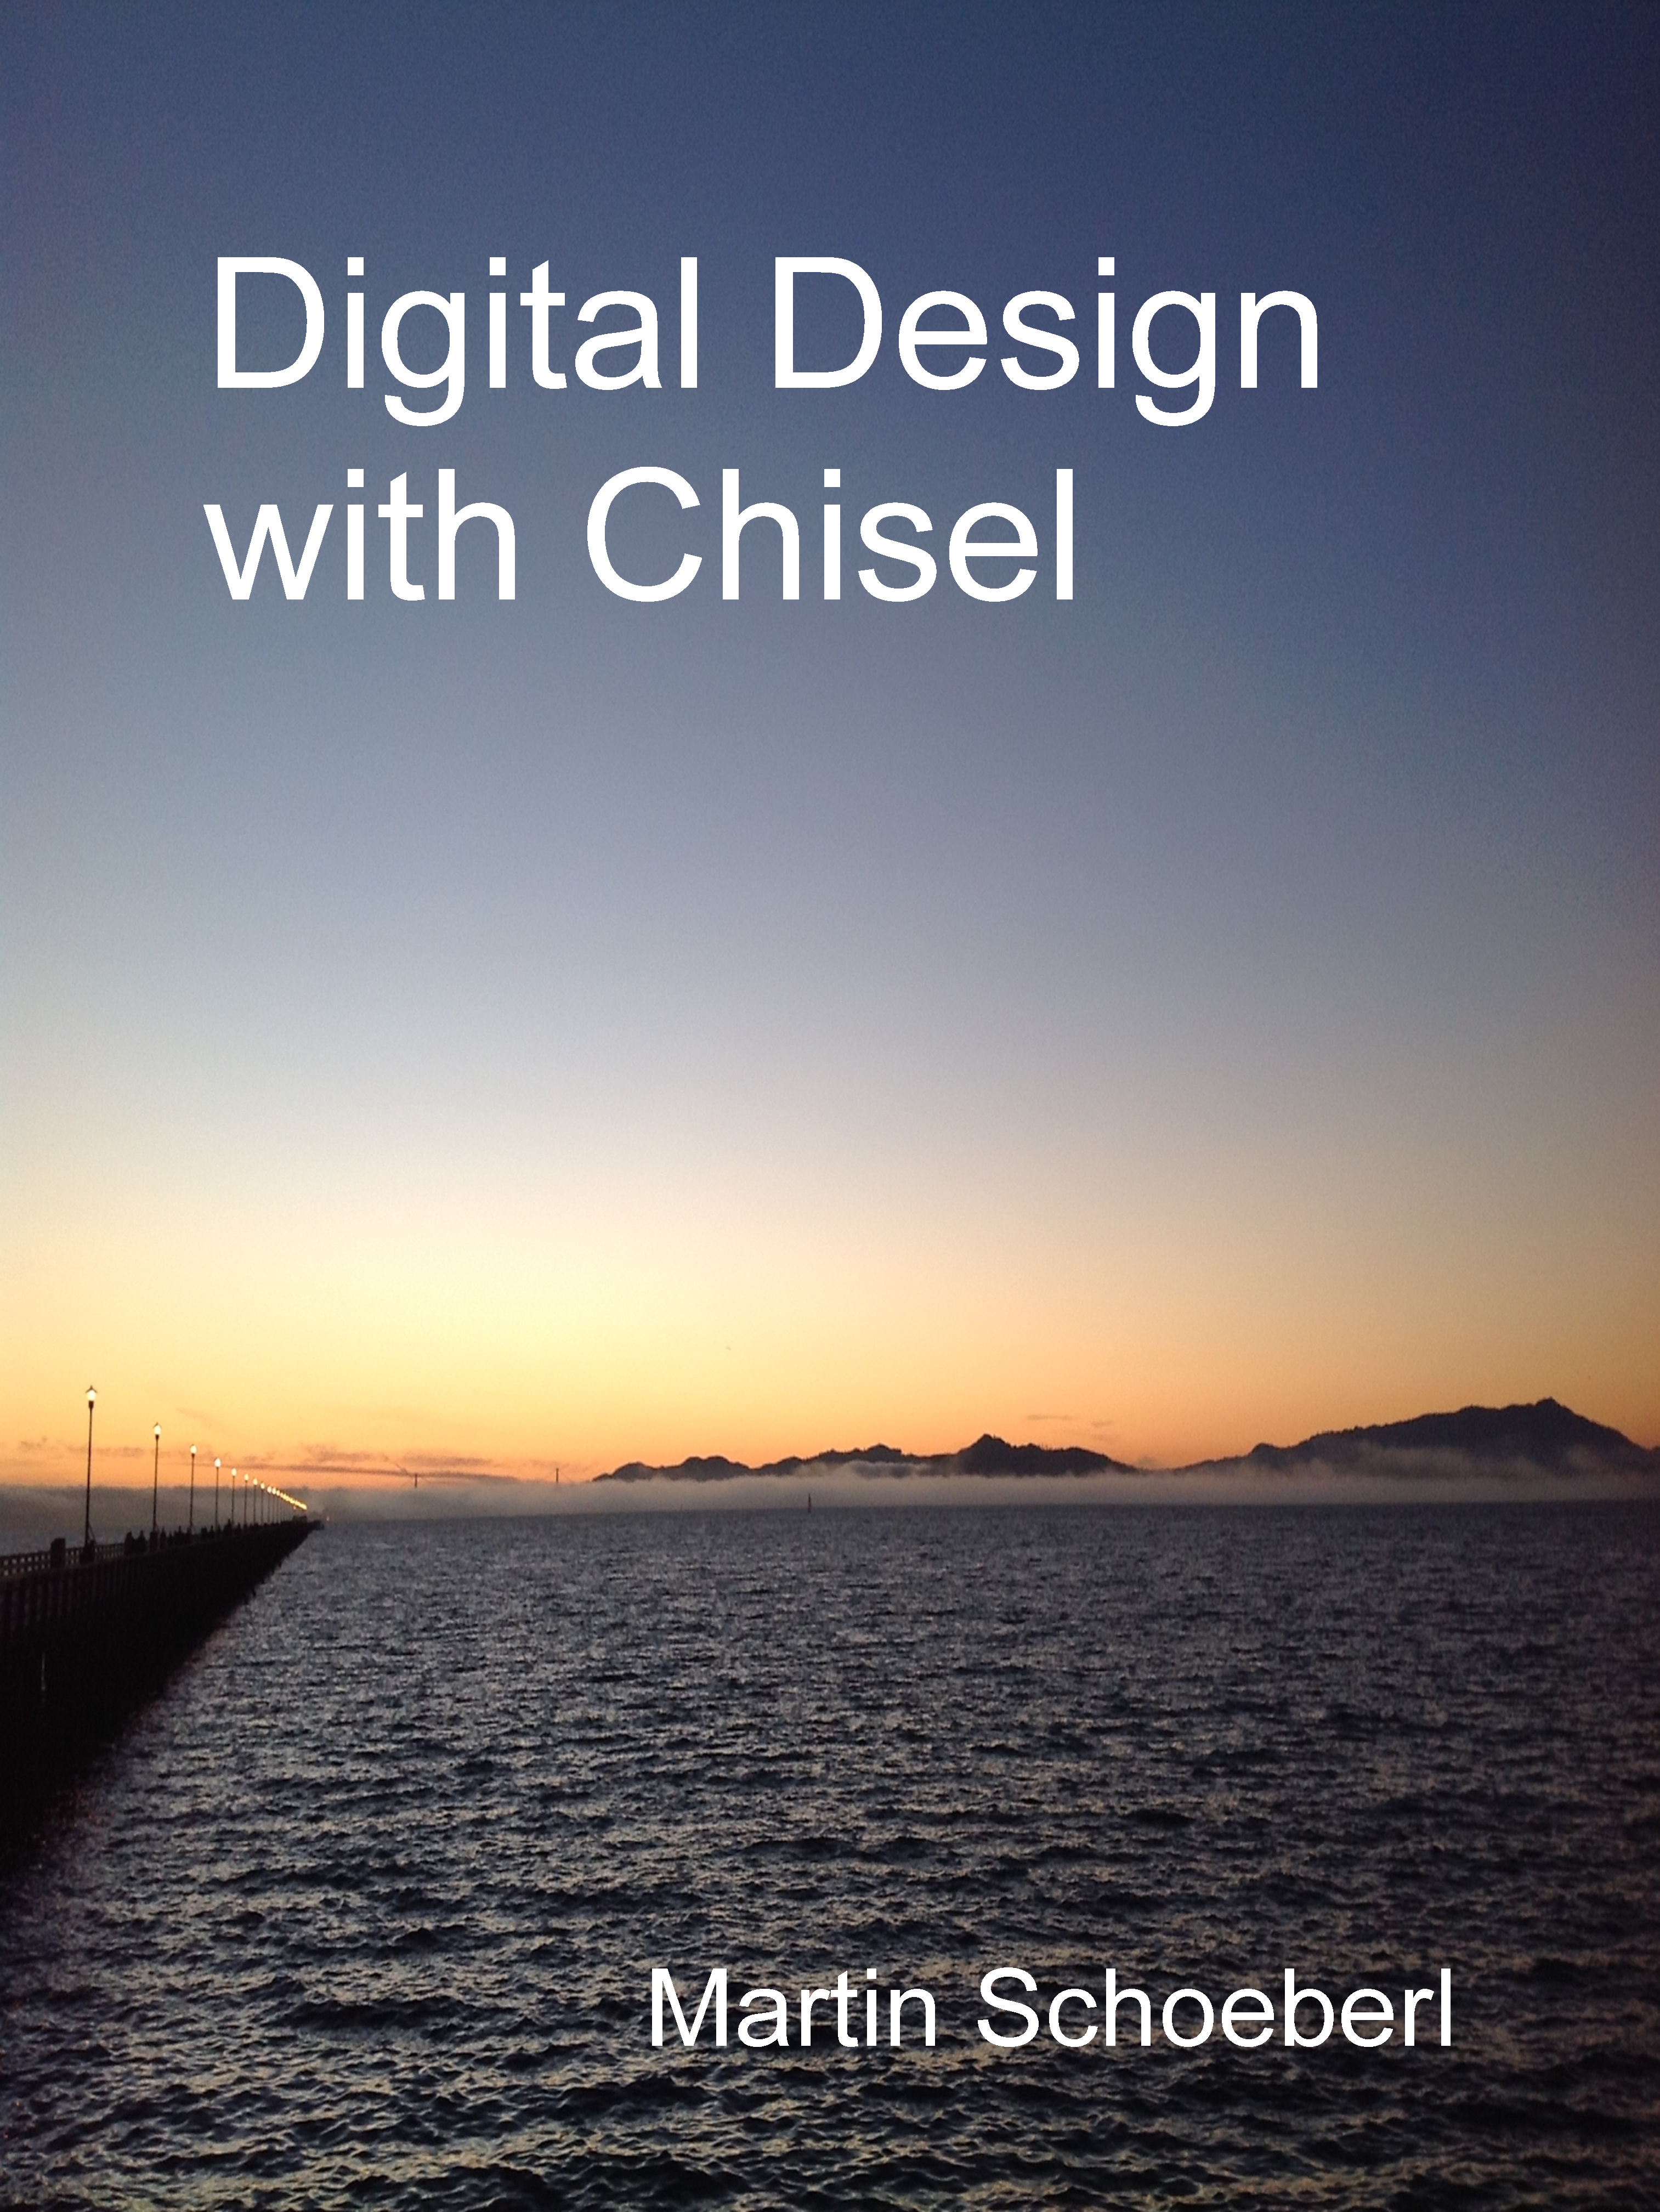
\includepdf{chisel-cover.pdf}
\newpage
\pagestyle{empty}
~
\newpage
\fi



\begin{flushleft}
\pagestyle{empty}
\ \\
\vspace{1cm}
{\usekomafont{title}\mdseries\huge Digital Design with Chisel}
\cleardoublepage
\end{flushleft}
\newpage


\begin{flushleft}
\pagestyle{empty}
\ \\
\vspace{1cm}
{\usekomafont{title}\Huge Digital Design with Chisel\\
\bigskip
\bigskip
\bigskip
\bigskip
\bigskip
%{\large\itshape Beta Edition}\\
\bigskip
{\usekomafont{title}\huge Martin Schoeberl}
\medskip\\
%{\large\itshape martin@jopdesign.com}

}

%\vspace{10cm} \emph{Version: \today}
\newpage
\end{flushleft}

\thispagestyle{empty}
\begin{flushleft}
{\small

%\lowertitleback{
Copyright \copyright{} 2016--2019 Martin Schoeberl
  \medskip\\
  \begin{tabular}{lp{.8\textwidth}}
    \raisebox{-12pt}{
\includegraphics[height=18pt]{figures/cc_by_sa}} &
     This work is licensed under a Creative Commons Attribution-ShareAlike
     4.0 International License.
     \url{http://creativecommons.org/licenses/by-sa/4.0/}\\
  \end{tabular}
%}

\medskip

Email: \url{martin@jopdesign.com}\\
Visit the source at \url{https://github.com/schoeberl/chisel-book}
\medskip

Published 2019 by Kindle Direct Publishing,\\
\url{https://kdp.amazon.com/}
\medskip
\medskip


\textbf{Library of Congress Cataloging-in-Publication Data}
\medskip

Schoeberl, Martin
\begin{quote}
Digital Design with Chisel\\
Martin Schoeberl\\
Includes bibliographical references.\\ \todo{and index. \\}
ISBN 9781689336031
\end{quote}

\bigskip


Manufactured in the United States of America.

Typeset by Martin Schoeberl.}
\end{flushleft}

\frontmatter

\phantomsection
\hypertarget{contents}{}
\tableofcontents


\begingroup
\let\cleardoublepage\clearpage
\listoffigures
\listoftables
\lstlistoflistings
\endgroup

%\chapter*{Foreword}
%
%Here comes the text.
%
%\bigskip
%
%Jonathan Bachrach, designer of Chisel

\chapter{Preface}

% This text goes on the backside of the book, and in Amazon description
This book is an introduction to digital design with the focus on using the hardware construction language Chisel. Chisel brings advances from software engineering, such as object-orientated and functional languages, into digital design.

This book addresses hardware designers and software engineers. Hardware designers, with knowledge of Verilog or VHDL, can upgrade their productivity with a modern language for their next ASIC or FPGA design. Software engineers, with knowledge of object-oriented and functional programming, can leverage their knowledge to program hardware, for example, FPGA accelerators executing in the cloud.

The approach of this book is to present small to medium-sized typical hardware components to explore digital design with Chisel.

% about me, backside

%Martin Schoeberl is Associate Professor at the Technical University of Denmark, where he is teaching digital electronics and computer architecture. His research interest is on hard real-time systems, time-predictable computer architecture, and real-time Java. He has more than 100 publications in peer reviewed journals, conferences, and books.

%Martin has been four times at UC Berkeley on research stays, where he has picked up Chisel and was in close contact with the developers of Chisel. He lead the research project T-CREST where most of the components have been written in Chisel.

\section*{Acknowledgements}

I want to thank everyone who has worked on Chisel for creating such
a cool hardware construction language. Chisel is so joyful to use and
therefore worth writing a book about.
I am thankful to the whole Chisel community, which is so welcoming and friendly
and never tired to answer questions on Chisel.

I would also like to thank my students in the last years of an advanced computer
architecture course where most of them picked up Chisel for the final project.
Thank you for moving out of your comfort zone and taking up the journey of
learning and using a bleeding-edge hardware description language.
Many of your questions have helped to shape this book.


\mainmatter

\chapter{Introduction}
\label{sec:intro}

This book is an introduction to digital system design using a modern hardware
construction language, \myref{https://chisel.eecs.berkeley.edu/}{Chisel}~\cite{chisel:dac2012}.
In this book, we focus on a higher abstraction level than usual in digital design books,
to enable you to build more complex, interacting digital systems in a shorter time.

This book and Chisel are targeting two groups of developers:
(1) hardware designers and (2) software programmers.
Hardware designers who are fluid in VHDL or Verilog and using other languages such as Python,
Java, or Tcl to generate hardware can move to a single hardware construction language
where hardware generation is part of the language and
Software programmers may become interested in hardware design,
e.g., as future chips from Intel will include programmable hardware to speed up programs.
It is perfectly fine to use Chisel as your first hardware description language.

Chisel brings advances in software engineering, such as object-orientated
and functional languages, into digital design.
Chisel does not only allow to express hardware at the register-transfer level
but allows you to write hardware generators.

Hardware is now commonly described with a hardware description language.
The time of drawing hardware components, even with CAD tools, is
over. Some high-level schematics can give an overview of the system but are
not intended to describe the system.
The two most common hardware description languages are Verilog and VHDL.
Both languages are old, contain many legacies, and have a moving line of what
constructs of the language are synthesizable to hardware.
Do not get me wrong: VHDL and Verilog are perfectly able to describe a hardware
block that can be synthesized into an
\myref{https://en.wikipedia.org/wiki/Application-specific_integrated_circuit}{ASIC}.
For hardware design in Chisel, Verilog serves as an intermediate language
for testing and synthesis.

This book is not a general introduction to hardware design and the fundamentals of it.
For an introduction of the basics in digital design, such as how to build a gate out of
CMOS transistors, refer to other digital design books.
However, this book intends to teach digital design at an abstraction level that is
current practice to describe ASICs or designs targeting
\myref{https://en.wikipedia.org/wiki/Field-programmable_gate_array}{FPGA}s.\footnote{As the author is more familiar with FPGAs
than ASICs as target technology, some design optimizations shown in this book are
targeting FPGA technology.}
As prerequisites for this book, we assume basic knowledge of
\myref{https://en.wikipedia.org/wiki/Boolean_algebra}{Boolean algebra} and the
\myref{https://en.wikipedia.org/wiki/Binary_number}{binary number system}.
Furthermore, some programming experience in any programming language
is assumed. No knowledge of Verilog or VHDL is needed.
Chisel can be your first programming language to describe digital hardware.
As the build process in the examples is based on \code{sbt} and \code{make}
basic knowledge of the command-line interface (CLI, also called terminal or
Unix shell) will be helpful.

Chisel itself is not a big language. The basic constructs fit on
\myref{https://chisel.eecs.berkeley.edu/doc/chisel-cheatsheet3.pdf}{one page}
and can be learned within a few days.
Therefore, this book is not a big book, as well.
Chisel is for sure smaller than VHDL and Verilog, which carry many legacies.
The power of Chisel comes from the embedding of Chisel within
\myref{https://www.scala-lang.org/}{Scala}, which itself in an expressive language.
Chisel inherits the feature from Scala being ``a language that grows on you''~\cite{Scala}.
However, Scala is not the topic of this book.
% We provide a short section on Scala for hardware designers, but
%A general introduction to Scala is better served by
The textbook by Odersky et al.~\cite{Scala} provides a general introduction
to Scala.
This book is a tutorial in digital design and the Chisel language; it is not
a Chisel language reference, nor is it a book on complete chip design.


All code examples shown in this book are extracted from complete programs
that have been compiled and tested. Therefore, the code shall not contain
any syntax errors. The code examples are available from the
\myref{https://github.com/schoeberl/chisel-book}{GitHub repository}
of this book.
Besides showing Chisel code, we have also tried to show useful designs and
principles of good hardware description style.

This book is optimized for reading on a laptop or tablet (e.g., an iPad).
We include links to further reading in the running text, mostly to
\myref{https://en.wikipedia.org/}{Wikipedia} articles.

\section{Installing Chisel and FPGA Tools}

Chisel is a Scala library, and the easiest way to install Chisel and Scala is
with \code{sbt}, the Scala build tool. Scala itself depends on the installation
of the \myref{https://www.oracle.com/technetwork/java/javase/downloads/jdk8-downloads-2133151.html}{Java JDK 1.8}.

On Mac OS X, with the packet manager \myref{https://brew.sh/}{Homebrew},
\code{sbt} is installed with:

\begin{verbatim}
$ brew install sbt
\end{verbatim}

\noindent For Ubuntu, which is based on Debian, programs are usually installed from a
Debian file (.deb). However, as of the time of this writing \code{sbt} is not
available as a ready to install package. Therefore, the installation process
is a little bit more involved:
\begin{verbatim}
echo "deb https://dl.bintray.com/sbt/debian /" | \
  sudo tee -a /etc/apt/sources.list.d/sbt.list
sudo apt-key adv --keyserver hkp://keyserver.ubuntu.com:80 \
  --recv 2EE0EA64E40A89B84B2DF73499E82A75642AC823
sudo apt-get update
sudo apt-get install sbt
\end{verbatim}

Chisel and Scala can also be installed and used under Windows.
\code{sbt} can be installed with a Windows installer, see:
\myref{https://www.scala-sbt.org/1.x/docs/Installing-sbt-on-Windows.html}{Installing sbt on Windows}.

To build hardware for an FPGA, you need a synthesize tool. The two major
FPGA vendors, Intel\footnote{former Altera} and Xilinx, provide free versions of
their tools that cover small to medium-sized FPGAs. Those medium-sized
FPGAs are large enough to build multicore RISC style processors.
Intel provides the \myref{https://www.altera.com/products/design-software/fpga-design/quartus-prime/download.html}{Quartus Prime Lite Edition} and Xilinx the
\myref{https://www.xilinx.com/products/design-tools/vivado/vivado-webpack.html}{Vivado Design Suite, WebPACK Edition}.

\section{Hello World}

Each book on a programming language shall start with a minimal example,
called the \emph{Hello World} example. Following code is the first approach:


\shortlist{src/main/scala/HelloScala.scala}


\noindent Compiling and executing this short program with \code{sbt}

\begin{chisel}
$ sbt "runMain HelloScala"
\end{chisel}

\noindent leads to the expected output of a Hello World program:

\begin{chisel}
[info] Running HelloScala
Hello Chisel World!
\end{chisel}

\noindent However, is this Chisel? Is this hardware generated to print a string?
No, this is plain Scala code and not a representative Hello World
program for a hardware design.

\section{Chisel Hello World}

What is then the equivalent of a Hello World program for a hardware design?
The minimal useful and visible design? A blinking LED is the hardware (or even
embedded software) version of Hello World. If a LED blinks, we are ready to
solve bigger problems!

\longlist{code/hello.txt}{A hardware Hello World in Chisel}{lst:chisel:hello}

Listing~\ref{lst:chisel:hello} shows a blinking LED, described in Chisel.
It is not important that you understand the details of this code example.
We will cover those in the following chapters. Just note that the circuit is
usually clocked with a high frequency, e.g., 50 MHz, and we need a counter
to derive timing in the Hz range to achieve a visible blinking. In the above
example, we count from 0 up to 25000000-1 and then toggle the blinking signal
(\code{blkReg := \textasciitilde blkReg}) and restart the counter (\code{cntReg := 0.U}).
That hardware then blinks the LED at 1~Hz.

\section{An IDE for Chisel}

This book makes no assumptions about your programming environment or editor to use.
Learning of the basics should be easy with just using \code{sbt} at the command line
and an editor of your choice. In the tradition of other books, all commands that you
shall type in a shell/terminal/CLI are preceded by a \code{\$} character, which you
shall not type in. As an example, here is the Unix \code{ls} command, which lists files in
the current folder:

\begin{verbatim}
$ ls
\end{verbatim}

That said, an integrated development environment (IDE), where a compiler is running in
the background, can speed up coding. As Chisel is a Scala library, all IDEs
that support Scala are also good IDEs for Chisel.
It is possible in \myref{https://www.eclipse.org/}{Eclipse} and
\myref{https://www.jetbrains.com/help/idea/discover-intellij-idea-for-scala.html}{IntelliJ}
to generate a project from the sbt project configuration in \code{build.sbt}.
You can create an Eclipse project via
\begin{verbatim}
$ sbt eclipse
\end{verbatim}
and import that project into Eclipse.\footnote{This function needs the Eclipse plugin for sbt.}
In IntelliJ you can create a new project from existing sources and then select from \code{build.sbt}.

\section{Source Access and eBook Features}

This book is open source and hosted at GitHub: \myref{https://github.com/schoeberl/chisel-book}{chisel-book}.
All Chisel code examples, shown in this book, are included in the repository.
The code compiles with a recent version of Chisel, and many examples also include a test bench.
We collect larger Chisel examples in the accompanying repository \myref{https://github.com/schoeberl/chisel-examples}{chisel-examples}. If you find an error or typo in the book, a GitHub pull request is the most convenient way to incorporate your improvement.
You can also provide feedback or comments for improvements by filing an issue on GitHub
or sending a plain, old school email.

This book is freely available as a PDF eBook and in classical printed form.
The eBook version features links to further resources
and \myref{https://www.wikipedia.org/}{Wikipedia} entries.
We use Wikipedia entries for background information (e.g., binary number system)
that does not directly fit into this book.
We optimized the format of the eBook for reading on a tablet, such as an iPad.

\section{Further Reading}

Here a list of further reading for digital design and Chisel:
\begin{itemize}
\item \myref{http://www.cambridge.org/es/academic/subjects/engineering/circuits-and-systems/digital-design-systems-approach}{Digital Design: A Systems Approach}, by William J. Dally and R. Curtis Harting,
is a modern textbook on digital design. It is available in two versions: using Verilog or VHDL as a hardware description language.
\end{itemize}

The official Chisel documentation and further documents are available online:

\begin{itemize}
\item The \myref{https://chisel.eecs.berkeley.edu/}{Chisel} home page is the official starting point to
download and learn Chisel.
\item The \myref{https://github.com/ucb-bar/chisel-tutorial}{Chisel Tutorial} provides a ready setup
project containing small exercises with testers and solutions.

\item The \myref{https://github.com/freechipsproject/chisel3/wiki}{Chisel Wiki} contains
a short users guide to Chisel and links to further information.
\item The \myref{https://github.com/freechipsproject/chisel-testers}{Chisel Testers} are in
their repository that contains a Wiki documentation.
\item The \myref{https://github.com/ucb-bar/generator-bootcamp}{Generator Bootcamp} is
a Chisel course focusing on hardware generators, as a Jupyter notebook
\item A \myref{https://github.com/ccelio/chisel-style-guide}{Chisel Style Guide} by Christopher Celio.
\end{itemize}

\section{Exercise}

Each chapter ends with a hands-on exercise. For the introduction exercise, we will use an
FPGA board to get one \myref{https://en.wikipedia.org/wiki/Light-emitting_diode}{LED} blinking.
As a first step clone (or fork) the \myref{https://github.com/schoeberl/chisel-examples}{chisel-examples}
repository from GitHub.
The Hello World example is in the folder \code{hello-world}, set up as
a minimal project. You can explore the Chisel code of the blinking LED
in \code{src/main/scala/Hello.scala}.
Compile the blinking LED with the following steps:

\begin{chisel}
$ git clone https://github.com/schoeberl/chisel-examples.git
$ cd chisel-examples/hello-world/
$ make
\end{chisel}

After some initial downloading of Chisel components, this will produce the Verilog file \code{Hello.v}.
Explore this Verilog file. You will see that it contains two inputs \code{clock} and \code{reset}
and one output \code{io\_led}. When you compare this Verilog file with the Chisel module,
you will notice that the Chisel module does not contain \code{clock} or \code{reset}.
Those signals are implicitly generated, and in most designs, it is convenient not to need to
deal with these low-level details. Chisel provides register components, and those
are connected automatically to \code{clock} and \code{reset} (if needed).

The next step is to set up an FPGA project file for the synthesize tool, assign the pins,
and compile\footnote{The real process is more elaborated with following steps: synthesizing the logic,
performing place and route, performing timing analysis, and generating a bitfile.
However, for the purpose of this introduction example we simply call it ``compile''
your code.} the Verilog code, and configure the FPGA with the resulting bitfile.
We cannot provide the details of these steps. Please consult the manual of
your Intel Quartus or Xilinx Vivado tool.
However, the examples repository contains some ready to use Quartus
projects in folder \code{quartus} for several popular FPGA boards (e.g., DE2-115).
If the repository contains support for your board, start Quartus, open the project,
compile it by pressing the \emph{Play} button, and configure the FPGA board
with the \emph{Programmer} button and one of the LEDs should blink.

{\bf Gratulation! You managed to get your first design in Chisel running in an FPGA!}

If the LED is not blinking, check the status of reset. On the DE2-115 configuration,
the reset input is connected to SW0.

Now change the blinking frequency to a slower or a faster value and
rerun the build process. Blinking frequencies and also blinking patterns
communicate different ``emotions''. E.g., a slow blinking LED signals that
everything is ok, a fast blinking LED signals an alarm state.
Explore which frequencies express best those two different emotions.

As a more challenging extension to the exercise, generate the following blinking pattern:
the LED shall be on for 200~ms every second. For this pattern, you might
decouple the change of the LED blinking from the counter reset.
You will need a second constant where you change the state of the
\code{blkReg} register. What kind of emotion does this pattern produce?
Is it alarming or more like a sign-of-live signal?




\chapter{Basic Components}

In this section, we introduce the basic components for digital design:
combinational circuits and flip-flops.
These essential elements can be combined to build larger, more interesting circuits.

\section{Signal Types and Constants}

Chisel provides three data types to describe signals, combinational logic, and registers:
\code{Bits}, \code{UInt}, and \code{SInt}. \code{UInt} and \code{SInt} extend \code{Bits},
and all three types represent a vector of bits. \code{UInt} gives this vector of
bits the meaning of an unsigned integer and \code{SInt} of a signed
integer.\footnote{The type \codefoot{Bits} in the current version of Chisel is missing operations and
therefore not very useful for user code.}
Chisel uses \myref{https://en.wikipedia.org/wiki/Two\%27s\_complement}{two's complement}
as signed integer representation.
Here is the definition for different types, an 8-bit \code{Bits}, an 8-bit unsigned integer, and a 10-bit
signed integer:

\shortlist{code/types.txt}

\noindent The width of a vector of bits is defined by a Chisel width type (\code{Width}).
The following expression casts the Scala integer \code{n} to a Chisel \code{width},
which is used for the definition of the \code{Bits} vector:

\shortlist{code/n_w.txt}

\noindent Constants can be defined by using a Scala integer and converting it to a Chisel type:

\shortlist{code/constants.txt}

\noindent Constants can also be defined with a width, by using the Chisel width type:

\shortlist{code/const_width.txt}

\noindent If you find the notion of 8.U and 4.W a little bit funny, consider it as a variant of an integer
constant with a type. This notation is similar to 8L, representing a long integer constant in C, Java, and Scala.

Chisel benefits from Scala's type inference and in many places type information can be left out.
The same is also valid for bit widths. In many cases, Chisel will automatically infer the correct width.
Therefore, a Chisel description of hardware is more concise and better readable than VHDL or
Verilog.

For constants defined in other bases than decimal, the constant is defined in a string with
a preceding \code{h} for hexadecimal (base 16), \code{o} for octal (base 8), and \code{b}
for binary (base 2). The following example shows the definition of constant 255 in different
bases. In this example we omit the bit width and Chisel infers the minimum width to fit
the constants in, in this case 8 bits.

\shortlist{code/const_base.txt}

\noindent The above code shows how to use an underscore to group digits in the
string that represents a constant. The underscore is ignored.

To represent logic values, Chisel defines the type \code{Bool}.
\code{Bool} can represent a \emph{true} or \emph{false} value.
The following code shows the definition of type \code{Bool} and the definition of
\code{Bool} constants, by converting the Scala Boolean constants \code{true}
and \code{false} to Chisel \code{Bool} constants.

\shortlist{code/bool.txt}


\section{Combinational Circuits}

Chisel uses \myref{https://en.wikipedia.org/wiki/Boolean_algebra}{Boolean algebra} operators,
as they are defined in C, Java, Scala, and several other programming languages,
to described combinational circuits: \code{\&} is the AND operator and \code{|} is
the OR operator.
Following line of code defines a circuit that combines signals \code{a} and \code{b} with \emph{and}
gates and combines the result with signal \code{c} with \emph{or} gates.

\shortlist{code/logic.txt}

\begin{figure}
  \centering
  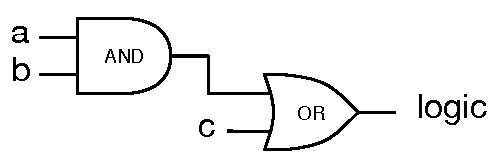
\includegraphics[scale=\scale]{figures/logic}
  \caption{Logic for the expression \code{(a \& b) | c}.
  The wires can be a single bit or multiple bits. The Chisel expression, and the schematics are the same.}
  \label{fig:logic}
\end{figure}


Figure~\ref{fig:logic} shows the schematic of this combinatorial expression.
Note that this circuit may be for a vector of bits and not only single wires
that are combined with the AND and OR circuits.

In this example, we do not define the type nor the width of signal \code{logic}.
Both are inferred from the type and width of the expression.
The standard logic operations in Chisel are:

\shortlist{code/bool_ops.txt}

\noindent The arithmetic operations use the standard operators:

\shortlist{code/arith_ops.txt}

\noindent The resulting width of the operation is the maximum width of the operators for
addition and subtraction, the sum of the two widths for the multiplication, and usually
the width of the numerator for divide and modulo operations.\footnote{The exact
details are available in the \myref{https://github.com/freechipsproject/firrtl/blob/master/spec/spec.pdf}{FIRRTL specification}.}

A signal can also first be defined as a \code{Wire} of some type. Afterward, we can assign a
value to the wire with the \code{:=} update operator.

\shortlist{code/wire.txt}

A single bit can be extracted as follows:
\shortlist{code/single_bit.txt}

\noindent A subfield can be extracted from end to start position:
\shortlist{code/sub_field.txt}

\noindent Bit fields are concatenated with \code{Cat}.
\shortlist{code/concat.txt}

Table~\ref{tab:operators} shows the full list of operators
(see also \myref{https://github.com/freechipsproject/chisel3/wiki/Builtin-Operators}{builtin operators}).
The Chisel operator precedence is determined by the evaluation order of the circuit,
which follows the \myref{https://docs.scala-lang.org/tour/operators.html}{Scala operator precedence}.
If in doubt, it is always a good praxis to use parentheses.\footnote{The operator precedence in
Chisel is a side effect of the hardware elaboration when the tree of hardware nodes
is created by executing the Scala operators. The Scala operator precedence is similar but
not identical to Java/C. Verilog has the same operator precedence as C, but VHDL
has a different one. Verilog has precedence ordering for logic operations, but in VHDL
those operators have the same precedence and are evaluated from left to right.}

Table~\ref{tab:functions} shows various functions defined on and for Chisel data types.

\begin{table}
 \centering
 \label{tab:operators}
  \begin{tabular}{lll}
    \toprule
    Operator & Description & Data types \\
    \midrule
    \code{* / \%} & multiplication, division, modulus & UInt, SInt \\
    \code{+ -} & addition, subtraction & UInt, SInt \\
    \code{=== =/=} & equal, not equal & UInt, SInt, returns Bool \\
    \code{> >= < <=} & comparison & UInt, SInt, returns Bool \\
    \code{<< >>} & shift left, shift right (sign extend on SInt) & UInt, SInt \\
    \code{\~} & NOT & UInt, SInt, Bool \\
    \code{\& | \^} & AND, OR, XOR & UInt, SInt, Bool \\
    \code{!} & logical NOT & Bool \\
    \code{\&\& ||} & logical AND, OR & Bool \\
    \bottomrule 
  \end{tabular} 
  \caption{Chisel defined hardware operators.}
\end{table}

\begin{table}
 \centering
 \label{tab:functions}
  \begin{tabular}{lll}
    \toprule
    Function & Description & Data types \\
    \midrule
    \code{v.andR v.orR v.xorR} & AND, OR, XOR reduction & UInt, SInt, returns Bool \\
    \code{v(n)} & extraction of a single bit & UInt, SInt \\
    \code{v(end, start)} & bitfield extraction & UInt, SInt \\
    \code{Fill(n, v)} & bitstring replication, n times & UInt, SInt \\
    \code{Cat(a, b, ...)} & bit field concatenation & UInt, SInt \\
    \bottomrule 
  \end{tabular} 
  \caption{Chisel defined hardware functions, invoked on \code{v}.}
\end{table}                                            
    

\subsection{Multiplexer}

A \myref{https://en.wikipedia.org/wiki/Multiplexer}{multiplexer} is a circuit that selects between alternatives.
In the most basic form, it selects between two alternatives. Figure~\ref{fig:mux} shows
such a 2:1 multiplexer, or mux for short. Depending on the value of the
select signal (\code{sel}) signal \code{y} will represent signal \code{a} or
signal \code{b}.

\begin{figure}
  \centering
  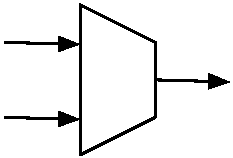
\includegraphics[scale=\scale]{figures/mux}
  \caption{A basic 2:1 multiplexer.}
  \label{fig:mux}
\end{figure}

A multiplexer can be built from logic.
However, as multiplexing  is such a standard operation, Chisel provides a multiplexer,

\shortlist{code/mux.txt}

\noindent where \code{a} is selected when the \code{sel} is \code{true.B}, otherwise \code{b}
is selected. The type of \code{sel} is a Chisel \code{Bool}; the inputs \code{a} and \code{b}
can be any Chisel base type or aggregate (bundles or vectors) as long as they are the same
type.

With logical and arithmetical operations and a multiplexer, every combinational
circuit can be described. However, Chisel provides further components and control abstractions
for a more elegant description of a combinational circuit, which are described in
a later chapter.

The second basic component needed to describe a digital circuit is a state element,
also called register, which is described next.

\section{Registers}

Chisel provides a register, which is a collection of
\myref{https://en.wikipedia.org/wiki/Flip-flop\_(electronics)\#D\_flip-flop}{D flip-flops}.
The register is implicitly connected to a global clock and is updated on the rising edge.
When an initialization value is provided at the declaration of the register,
it uses a synchronous reset connected to a global reset signal.
A register can be any Chisel type that can be represented as a collection of bits.
Following code defines an 8-bit register, initialized with 0 at reset:

\shortlist{code/register.txt}

\noindent An input is connected to the register with the \code{:=} update operator and
the output of the register can be used just with the name in an expression:

\shortlist{code/reg_con.txt}

\noindent A register can also be connected to its input at the definition:

\shortlist{code/reg_next.txt}

\noindent A register can also be connected to its input and a constant as
initial value at the definition:

\shortlist{code/reg_both.txt}

\noindent To distinguish between signals representing combinational logic and registers,
a common practice is to postfix register names with \code{Reg}.
Another common practice, coming from Java and Scala, is to use
\myref{https://en.wikipedia.org/wiki/Camel_case}{camelCase} for
identifier consisting of several words. The convention is to start
functions and variables with a lower case and classes (types) with
an upper case.

\subsection{Counting}

Counting is a fundamental operation in digital systems. On might count events.
However, more often counting is used to define a time interval. Counting the
clock cycles and triggering an action when the time interval has expired.

A simple approach is counting up to a value. However, in computer science,
and digital design, counting starts at 0. Therefore, if we want to count till
10, we count from 0 to 9. The following code shows such a counter that counts
till 9 and wraps around to 0 when reaching 9.

\shortlist{code/counter.txt}

\section{Structure with Bundle and Vec}

Chisel provides two constructs to group related signals: (1) a \code{Bundle} to group
signals of different types and (2) a \code{Vec} to represent an indexable collection of signals
of the same type.
\code{Bundle}s and \code{Vec}s can be arbitrarily nested.


A Chisel bundle groups several signals. The entire bundle can be referenced
as a whole, or individual fields can be accessed by their name.
We can define a bundle (collection of signals) by defining a class that
extends \code{Bundle} and list the fields as \code{val}s within the constructor block.

\shortlist{code/bundle.txt}

\noindent To use a bundle, we create it with \code{new} and wrap it into a \code{Wire}.
The fields are accessed with the dot notation:

\shortlist{code/bundle_use.txt}

Dot notation is common in object-oriented languages, where \code{x.y} means
\code{x} is a reference to an object and \code{y} is a field of that object.
As Chisel is object-oriented, we use dot notation to access fields in a bundle.
A bundle is similar to a \code{struct} in C, a \code{record} in VHDL, or a
\code{struct} in SystemVerilog.
A bundle can also be referenced as a whole:

\shortlist{code/bundle_ref.txt}

A Chisel \code{Vec} represents a collection of signals of the same type (a vector).
Each element can be accessed by an index. A Chisel \code{Vec} is similar
to array data structures in other programing languages.\footnote{The name \codefoot{Array}
is already used in Scala.}
A \code{Vec} is created by calling the constructor with two parameters: the
number of elements and the type of the elements. A combinational \code{Vec}
needs to be wrapped into a \code{Wire}

\shortlist{code/vec.txt}

\noindent Individual elements are accessed with \code{(index)}.

\shortlist{code/vec_access.txt}

A vector wrapped into a \code{Wire} is a multiplexer.
We can also wrap a vector into a register to define an array of registers.
Following example defines a register file for a processor; 32 registers
each 32-bits wide, as for a classic 32-bit 
\myref{https://en.wikipedia.org/wiki/Reduced_instruction_set_computer}{RISC}
processor, like the 32-bit version of \myref{https://en.wikipedia.org/wiki/RISC-V}{RISC-V}.

\shortlist{code/reg_file.txt}

\noindent An element of that register file is accessed with an index and used as a normal register.

\shortlist{code/reg_file_access.txt}

We can freely mix bundles and vectors. When creating a vector with a bundle
type, we need to pass a prototype for the vector fields. Using our
\code{Channel}, which we defined above, we can create a vector of channels with:

\shortlist{code/vec_bundle.txt}

\noindent A bundle may as well contain a vector:

\shortlist{code/bundle_vec.txt}

When we want a register of a bundle type that needs a reset value,
we first create a \code{Wire} of that bundle, set the individual fields
as needed, and then passing this bundle to a \code{RegInit}:

\shortlist{code/bundle_reg_init.txt}

With combinations of \code{Bundle}s and \code{Vec}s we can define our own data
structures, which are powerful abstractions.

\section{Chisel Generates Hardware}

After seeing some initial Chisel code, it might look similar to classic programming
languages such as Java or C. However, Chisel (or any other hardware description
language) does define hardware components. While in a software program one
line of code after the other is executed, in hardware all lines of code
\emph{execute in parallel}.

It is essential to keep in mind that Chisel code does generate hardware.
Try to imagine, or draw on a sheet of paper, the individual blocks that
are generated by your Chisel circuit description.
Each creation of a component adds hardware; each assignment statement
generates gates and/or flip-flops.

More technically, when Chisel executes your code it runs as a Scala program, and
by executing the Chisel statements, it \emph{collects} the hardware components
and connects those nodes. This network of hardware nodes is the hardware,
which can spill out Verilog code for ASIC or FPGA synthesis or can be
tested with a Chisel tester.
The network of hardware nodes is what is executed in fully parallel.

For a software engineer imagine this immense parallelism that you can
create in hardware without needing to partition your application into threads
and getting the locking correct for the communication.


\section{Exercise}

In the introduction you implemented a blinking LED on an FPGA board
(from \myref{https://github.com/schoeberl/chisel-examples}{chisel-examples}), which is a reasonable
hardware \emph{Hello World} example. It used only internal state, a single LED output, and no input.
Copy that project into a new folder and extend it by adding some inputs to the \code{io} \code{Bundle}
with \code{val sw = Input(UInt(2.W))}.

\shortlist{code/basic_exercise.txt}

\noindent For those switches, you also need to assign the pin names for the FPGA board.
You can find examples of pin assignments in the Quartus project files of the ALU project
(e.g., for the \myref{https://github.com/schoeberl/chisel-examples/blob/master/quartus/altde2-115/alu.qsf}{DE2-115
FPGA board}).

When you have defined those inputs and the pin assignment, start with a simple test:
drop all blinking logic from the design and connect one switch to the LED output;
compile and configure the FPGA device. Can you switch the LED on an off with the switch?
If yes, you have now inputs available. If not, you need to debug your FPGA configuration.
The pin assignment can also be done with the GUI version of the tool.

Now use two switches and implement one of the basic combinational functions,
e.g., AND two switches and show the result on the LED. Change the function.
The next step involves three input switches to implement a multiplexer: one acts as
a select signal, and the other two are the two inputs for the 2:1 multiplexer.

Now you have been able to implement simple combinational functions and test them
in real hardware in an FPGA. As a next step, we will take a first look at how the build
process works to generate an FPGA configuration. Furthermore, we will also
explore a simple testing framework from Chisel, which allows you to test circuits
without configuring an FPGA and toggle switches.

\chapter{Build Process and Testing}

To get started with more interesting Chisel code we first need to learn how to compile
Chisel programs, how to generate Verilog code for execution in an FPGA, and how
to write tests for debugging and to verify that our circuits are correct.

Chisel is written in Scala, so any build process that supports Scala is possible
with a Chisel project. One popular build tool for Scala is \myref{https://www.scala-sbt.org/}{sbt},
which stands for the Scala interactive build tool.
Besides driving the build and test process, \code{sbt} also downloads the correct
version of Scala and the Chisel libraries.

\section{Building your Project with sbt}

The Scala library that represents Chisel and the Chisel testers are automatically
downloaded during the build process from a Maven repository.
The libraries are referenced by \code{build.sbt}. It is possible to configure \code{build.sbt}
with \code{latest.release} to always use the most actual version of Chisel.
However, this means on each build the version is looked up from the Maven
repository. This lookup needs an Internet connection for the build to succeed.
Better use a dedicated version of Chisel and all other Scala libraries in your \code{build.sbt}.
Maybe sometimes it is also good to be able to write hardware code and test it without an Internet connection.
For example, it is cool to do hardware design on a plane.

\subsection{Source Organization}

\code{sbt} inherits the source convention from the \myref{https://maven.apache.org/}{Maven}
build automation tool. Maven also organizes repositories of open-source Java libraries.\footnote{That is
also the place where you downloaded the Chisel library on your first build:
\url{https://mvnrepository.com/artifact/edu.berkeley.cs/chisel3}.}

\begin{figure}
\dirtree{%
.1 project.
.2 src.
.3 main.
.4 scala.
.5 package.
.6 sub-package.
.3 test.
.4 scala.
.5 package.
.2 target.
.2 generated.
}
\caption{Source tree of a Chisel project (using \code{sbt})}
\label{fig:folders}
\end{figure}

Figure~\ref{fig:folders} shows the organization of the source tree of a typical Chisel project.
The root of the project is the project home, which contains \code{build.sbt}.
It may also include a \code{Makefile} for the build process, a README, and a LICENSE file.
Folder \code{src} contains all source code. From there it is split between \code{main},
containing the hardware sources and \code{test} containing testers.
Chisel inherits from Scala, which inherits from Java the organization of source
in \myref{https://en.wikipedia.org/wiki/Java_package}{packages}.
Packages organize your Chisel code into namespaces. Packages can also contain
sub-packages.
The folder \code{target} contains the class files and other generated files.
I recommend to also use a folder for generated Verilog files, which is usually
call \code{generated}.


To use the facility of namespaces in Chisel, you need to declare that a class/module
is defined in a package, in this example in \code{mypacket}:

\shortlist{code/packet.txt}

\noindent Note that in this example we see the import of the \code{chisel3} packet
to use Chisel classes.

To use the module \code{Abc} in a different context (packet name space),
the components of packet \code{mypacket} need to be imported. The underscore
(\_) acts as wildcard, meaning that all classes of \code{mypacket} are imported.

\shortlist{code/usepacket.txt}

\noindent It is also possible to not import all types from \code{mypacket},
but use the fully qualified name \code{mypack.Abc} to refer to the module
\code{Abc} in packet \code{mypack}.

\shortlist{code/usepacket2.txt}

\noindent It is also possible to import just a single class and create an instance of it:

\shortlist{code/usepacket3.txt}


\subsection{Running sbt}

A Chisel project can be compiled and executed with a simple \code{sbt} command:

\begin{verbatim}
$ sbt run
\end{verbatim}

This command will compile all your Chisel code from the source tree and searches
for classes that contain an \code{object} that includes a \code{main} method, or simpler
that extends \code{App}. If there is more than one such object, all objects are listed and
one can be selected.
You can also directly specify the object that shall be executed as a parameter to \code{sbt}:

\begin{verbatim}
$ sbt "runMain mypacket.MyObject"
\end{verbatim}

Per default \code{sbt} searches only the \code{main} part of the source tree and not
the \code{test} part.\footnote{This is a convention form Java/Scala that the test folder contains
unit tests and not objects with a \codefoot{main}.} However, Chisel testers, as described here,
contain a \code{main}, but shall be placed in the \code{test} part of the source tree.
To execute a \code{main} in the tester tree use following \code{sbt} command:

\begin{verbatim}
$ sbt "test:runMain mypacket.MyTester"
\end{verbatim}

Now that we know the basic structure of a Chisel project and how to compile and run it
with \code{sbt}, we can continue with a simple testing framework.
    
\section{Testing with Chisel}

Tests of hardware designs are usually called \myref{https://www.xilinx.com/support/documentation/sw_manuals/xilinx10/isehelp/ise_c_simulation_test_bench.htm}{test benches}.
The test bench instantiates the design under test (DUT), drives input ports, observes output ports,
and compares them with expected values.

Chisel provides test benches in the form of a \code{PeekPokeTester}.
One strength of Chisel is that it can use the full power of Scala to write those
test benches. One can, for example, code the expected functionality of the hardware
in a software simulator and compare the simulation of the hardware with the
software simulation. This method is very efficient when testing an implementation
of a processor~\cite{lipsi:arcs2018}.

To use the \code{PeekPokeTester}, following packages need to be imported:

\shortlist{code/test_import.txt}

\noindent Testing a circuit contains (at least) three components: (1) the device under test (often
called DUT), (2) the testing logic, also called test bench, and (3) the tester objects
that contains the \code{main} function to start the testing.

The following code shows our simple design under test. It contains two input
ports and one output port, all with a 2-bit width. The circuit does a bit-wise AND
to it returns on the output:

\shortlist{code/test_dut.txt}

\noindent The test bench for this DUT extends \code{PeekPokeTester} and has
the DUT as a parameter for the constructor:

\shortlist{code/test_bench_simple.txt}

\noindent A \code{PeekPokeTester} can set input values with \code{poke()} and
read back output values with \code{peek()}. The tester advances the simulation by one
step (= one clock cycle) with \code{step(1)}.
We can print the values of the outputs with \code{println()}.

The test is created and run with the following tester main:

\shortlist{code/test_main_simple.txt}

\noindent When you run the test, you will see the results printed to the terminal
(besides other information):

\begin{verbatim}
[info] [0.004] SEED 1544207645120
[info] [0.008] Result is: 0
[info] [0.009] Result is: 2
test DeviceUnderTest Success: 0 tests passed in 7 cycles
taking 0.021820 seconds
[info] [0.010] RAN 2 CYCLES PASSED
\end{verbatim}

\noindent We see that 0 AND 1 results in 0; 3 AND 2 results in 2.
Besides manually inspecting printouts, which is an excellent starting point, we can also
express our expectations in the test bench itself with \code{expect()},
having the output port and the expected value as parameters.
The following example shows testing with \code{expect()}:

\shortlist{code/test_bench.txt}

\noindent Executing this test does not print out any values from the hardware,
but that all tests passed as all expect values are correct.

\begin{verbatim}
[info] [0.001] SEED 1544208437832
test DeviceUnderTest Success: 2 tests passed in 7 cycles
taking 0.018000 seconds
[info] [0.009] RAN 2 CYCLES PASSED
\end{verbatim}

\noindent A failed test, when either the DUT or the test bench contains an error,
produces an error message describing the difference between the expected and actual
value. In the following, we changed the test bench to expect a 4, which is an error:

\begin{verbatim}
[info] [0.002] SEED 1544208642263
[info] [0.011] EXPECT AT 2   io_out got 0 expected 4 FAIL
test DeviceUnderTest Success: 1 tests passed in 7 cycles
taking 0.022101 seconds
[info] [0.012] RAN 2 CYCLES FAILED FIRST AT CYCLE 2
\end{verbatim}

In this section, we described the basic testing facility with Chisel for simple tests.
However, in Chisel, the full power of Scala is available to write testers.
\todo{Have a link to the not yet written section for: We will show these possibilities later.}

\subsection{Using ScalaTest}

\myref{http://www.scalatest.org/}{ScalaTest} is a testing tool for Scala (and Java),
which we can use to run Chisel testers.
To use it, include the library in your \code{build.sbt} with the following line:

\begin{verbatim}
libraryDependencies += "org.scalatest" %% "scalatest" % "3.0.5" % "test"
\end{verbatim}

\noindent Tests are usually found in \code{src/test/scala} and can be run with:

\begin{verbatim}
$ sbt test
\end{verbatim}

\noindent A minimal test (a testing hello world) to test a Scala Integer
addition:

\shortlist{code/scalatest_hello_world.txt}

\noindent Although Chisel testing is more heavyweight than unit testing of Scala programs,
we can wrap a Chisel test into a ScalaTest class. For the \code{Tester} shown
before this is:

\shortlist{code/scalatest_simple.txt}

The main benefit of this exercise is to be able to run all tests with a simple
\code{sbt test} (instead of a running \code{main}). You can run just a single
test with \code{sbt}, as follows:

\begin{verbatim}
$ sbt "testOnly SimpleSpec"
\end{verbatim}

\section{Exercises}

For this exercise, we will revisit the blinking LED from
\myref{https://github.com/schoeberl/chisel-examples}{chisel-examples}
and explore Chisel testing. \todo{Also use the ALU example.}

\subsection{A Minimal Project}

First, let us find out what a minimal Chisel project is. Explore the files in the
\myref{https://github.com/schoeberl/chisel-examples/tree/master/hello-world}{Hello World}
example.
The \code{Hello.scala} is the single hardware source file.
It contains the hardware description of the blinking LED (\code{class Hello})
and an \code{App} that generates the Verilog code.

Each file starts with the import of Chisel and related packages:

\shortlist{code/import.txt}

\noindent Then follows the hardware description, as shown in Listing~\ref{lst:chisel:hello}.
To generate the Verilog description, we need an application. A Scala object that \code{extends App}
is an application that implicitly generates the main function where the application starts.
The only action of this application is to create a new \code{HelloWorld} object and pass it
to the Chisel driver \code{execute} function. The first argument is an array of Strings,
where build options can be set (e.g., the output folder). The following code will
generate the Verilog file \code{Hello.v}.

\shortlist{code/generate.txt}

\noindent Run the generation of the example manually with

\begin{chisel}
$ sbt "runMain Hello"
\end{chisel}

and explore the generated \code{Hello.v} with an editor. The generated Verilog code may not be
very readable, but we can find out some details. The file starts with a module \code{Hello},
which is the same name as our Chisel module. We can identify our LED port as
\code{output io\_led}. Pin names are the Chisel names with a prepended \code{io\_}.
Besides our LED pin, the module also contains \code{clock} and \code{reset} input signals.
Those two signals are added automatically by Chisel.

Furthermore, we can identify the definition of our two registers \code{cntReg} and \code{blkReg}.
We may also find the reset and update of those registers at the end of the module definition.
Note, that Chisel generates a synchronous reset.

For \code{sbt} to be able to fetch the correct Scala compiler and the Chisel library,
we need a \code{build.sbt}:

\begin{chisel}
scalaVersion := "2.11.7"

resolvers ++= Seq(
  Resolver.sonatypeRepo("snapshots"),
  Resolver.sonatypeRepo("releases")
)

libraryDependencies += "edu.berkeley.cs" %% "chisel3" % "3.1.2"
\end{chisel}

\noindent Note that in this example, we have a concrete Chisel version number to avoid checking on
each run for a new version (which will fail if we are not connected to the Internet,
e.g., when doing hardware design during a flight).
Change the \code{build.sbt} configuration to use the latest Chisel version by changing the
library dependency to

\begin{chisel}
libraryDependencies += "edu.berkeley.cs" %% "chisel3" % "latest.release"
\end{chisel}

\noindent and rerun the build with \code{sbt}. Is there a newer version of Chisel
available and will it be automatically downloaded?

For convenience, the project also contains a \code{Makefile}.
It just contains the \code{sbt} command, so we do not need to remember it and
can generate the Verilog code with:

\begin{chisel}
make
\end{chisel}

%The project also contains a
%\myref{https://github.com/schoeberl/chisel-examples/blob/master/hello-world/verilog/hello_top.v}{Verilog top level},
%which wires the reset signal to 0.
%This works for our example in an FPGA, as registers usually power up 0.
Besides a \code{README} file, the example project also contains project
files for different FPGA board. E.g., in
\myref{https://github.com/schoeberl/chisel-examples/tree/master/hello-world/quartus/altde2-115}{quartus/altde2-115} 
you can find the two project files to define a Quartus project for the DE2-115 board.
The main definitions (source files, device, pin assignments) can be found in a plain text file
\myref{https://github.com/schoeberl/chisel-examples/blob/master/hello-world/quartus/altde2-115/hello.qsf}{hello.qsf}.
Explore the file and find out which pins are connected to which signals.
If you need to adapt the project to a different board, there is where the changes are applied.
If you have Quartus installed, open that project, compile with the green \emph{Play} button,
and then configure the FPGA.

Note that the \emph{Hello World} is a minimal Chisel project.
More realistic projects have their source files organized in packages and contain testers.
The next exercise will explore such a project.

\subsection{A Testing Exercise}

In the last chapter's exercise, you have extended the blinking LED example with some input
to build an AND gate and a multiplexer and run this hardware in an FPGA.
We will now use this example and test the functionality with a Chisel tester
to automate testing and also to be independent of an FPGA.
Use your designs from the previous chapter and add a Chisel tester to test the functionality.
Try to enumerate all possible inputs and test the output with \code{except()}.

Testing within Chisel can speed up the debugging of your design.
However, it is always a good idea to synthesize your design for an FPGA and run tests
with the FPGA. There you can perform a reality check on the size of your design (usually
in LUTs and flip-flops) and your performance of your design in maximum clocking frequency.
As a reference point, a textbook style pipelined RISC processor may consume about 3000
4-bit LUTs and may run around 100~MHz in a low-cost FPGA (Intel Cyclone or
Xilinx Spartan).


\chapter{Components}

\begin{figure}
  \centering
  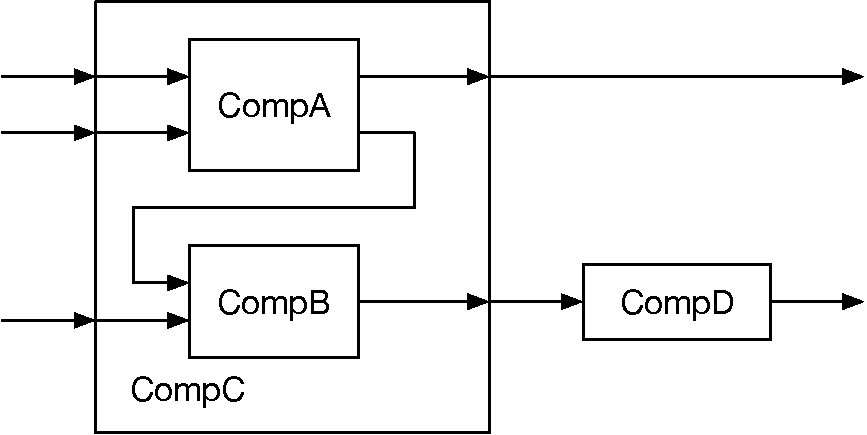
\includegraphics[scale=\scale]{figures/components}
  \caption{A design consisting of a hierarchy of components.}
  \label{fig:components}
\end{figure}


A larger digital design is structured into a set of components, often in
a hierarchical way. Each component has an interface with input and output
wires, usually called ports. These are similar to input and output pins on an integrated circuit (IC).
Components are connected by wiring up the inputs and outputs.
Components may contain subcomponents to build the hierarchy.
The outermost component, which is connected to physical pins
on a chip, is called the top-level component.

Figure~\ref{fig:components} shows an example design. Component C has
three input ports and two output ports. The component itself is assembled out
of two subcomponents: B and C, which are connected to the inputs and
outputs of C. One output of A is connected to an input of B.
Component D is at the same hierarchy level as component C and connected
to it.

In this chapter, we will explain how components are described in Chisel and
provide several examples of standard components.
Those standard components serve two purposes: (1) they provide examples
of Chisel code and (2) they provide a library of components ready to be reused
in your design.

\section{Components in Chisel are Modules}

Hardware components are called modules in Chisel. Each module extends
the class \code{Module} and contains a field \code{io} for the interface.
The interface is defined by a \code{Bundle} that is wrapped into a call to \code{IO()}.
The \code{Bundle} contains fields to represent input and output ports of
the module. The direction is given by wrapping a field into either a call to \code{Input()}
or \code{Output()}. The direction is from the view of the component itself.

The following code shows the definition of the two example components A and B from
Figure~\ref{fig:components}:

\shortlist{code/components_ab.txt}

\noindent Component A has two inputs, named \code{a} and \code{b}, and two
outputs, named \code{x} and \code{y}. For the ports of component B
we chose the names \code{in1}, \code{in2}, and \code{out}.
All ports use an unsigned integer (\code{UInt}) with a bit width of 8.
As this example code is about connecting components and building a
hierarchy, we do not show any implementation within the components.
The implementation of the component is written at the place where
the comments states ``function of X''.
As we have no function associated with those example components,
we used generic port names. For a real design use descriptive
port names, such as \code{data}, \code{valid}, or \code{ready}.

Component C has three input and two output ports. It is built out of
components A and B. We show how A and B are connected to the ports
of C and also the connection between an output port of A and an
input port of B:

\shortlist{code/components_c.txt}

Components are created with \code{new}, e.g., \code{new CompA()}, and need to be wrapped
into a call to \code{Module()}. The reference to that module is stored in a local variable,
in this example \code{val compA = Module(new CompA())}.

With this reference, we can access the IO ports by dereferencing the \code{io} field of the module
and the individual fields of the IO \code{Bundle}.

The simplest component in our design has just an input port, named \code{in}, and
an output port named \code{out}.

\shortlist{code/components_d.txt}

The final missing piece of our example design is the top-level component, which itself
is assembled out of components C and D:

\shortlist{code/components_top.txt}

Good component design is similar to the good design of functions or methods in
software design. One of the main questions is how much functionality shall we put into
a component and how large should a component be. The two extremes are tiny
components, such an adder, and huge components, such as a full microprocessor,

Beginners in hardware design often start with tiny components.
The problem is that digital design books use tiny components to show the principles.
But the sizes of the examples (in those books, and also in this book) is small
to fit into a page and to not distract by too many details.

The interface to a component is a little bit verbose (with types, names, directions,
IO construction). As a rule of thumb, I would propose that the core of the component,
the function, should be at least as long as the interface of the component.

For tiny components, such as a counter, Chisel provides a more lightweight
way to describe them as functions that return hardware.


\section{An Arithmetic Logic Unit}

One of the central components for circuits that compute, e.g., a microprocessor, is an
\myref{https://en.wikipedia.org/wiki/Arithmetic_logic_unit}{arithmetic-logic unit},
or ALU for short. Figure~\ref{fig:alu} shows the symbol of an ALU.

\begin{figure}
  \centering
  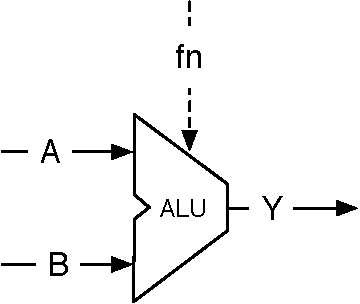
\includegraphics[scale=\scale]{figures/alu}
  \caption{An arithmetic logic unit, or ALU for short.}
  \label{fig:alu}
\end{figure}

The ALU has two data inputs, labeled \code{A} and \code{B} in the figure, one function input \code{fn},
and an output, labeled {Y}. The ALU operates on \code{A} and \code{B} and provides the result
at the output. The input \code{fn} selects the operation on \code{A} and \code{B}.
The operations are usually some arithmetic, such as addition and subtraction, and some logical
functions such as and, or, xor. That's why it is called ALU.

The function input \code{fn} selects the operation. The ALU is usually a combinational
circuit without any state elements. An ALU might also have additional outputs to signal properties
of the result, such as zero or the sign.

The following code shows an ALU with 16-bit inputs and outputs that supports: addition, subtraction, or, and and
operation, selected by a 2-bit \code{fn} signal.

\shortlist{code/components_alu.txt}

\noindent In this example, we use a new Chisel construct, the \code{switch/is} construct to describe
the table that selects the output of our ALU.
To use this utility function, we need to import another Chisel package:

\shortlist{code/components_util.txt}

\section{Bulk Connections}

For connecting components with multiple IO ports, Chisel provides the
bulk connection operator \code{<>}. This operator connects parts of bundles
in both directions. Chisel uses the names of the leave fields for the connection.
If a name is missing, it is not connected.

As an example, let us assume we build a pipelined processor. The fetch
stage has a following interface:
\shortlist{code/bundle_fetch.txt}

\noindent The next stage is the decode stage.
\shortlist{code/bundle_decode.txt}

\noindent The final stage of our simple processor is the execute stage.
\shortlist{code/bundle_execute.txt}

To connect all three stages we need just two \code{<>} operators.
We can also connect the port of a submodule with the parent module.
\shortlist{code/bundle_connect.txt}


\section{Lightweight Components with Functions}

Modules are the general way to structure your hardware description.
However, there is some boilerplate code when declaring a module and when instantiating and
connecting it.
A lightweight way to structure your hardware is to use functions.
Scala functions can take Chisel (and Scala) parameters and return generated hardware.
As a simple example, we generate an adder:

\shortlist{code/components_fn_def.txt}

\noindent We can then create two adders by simply calling the function \code{adder}.

\shortlist{code/components_fn_use.txt}

\noindent Note that this is a \emph{hardware generator}. You are not executing any add operation
during elaboration, but create two adders (hardware instances). The adder is an artificial example
to keep it simple. Chisel has already an adder generation function, like \code{+(that: UInt)}.

Functions as lightweight hardware generators can also contain state (including a register).
Following example returns a one clock cycle delay element (a register).
If a function has just a single statement, we can write it in one line and omit the curly
braces ({}).

\shortlist{code/components_fn_delay.txt}

\noindent By calling the function with the function itself as parameter, this generated a two
clock cycle delay.

\shortlist{code/components_fn_2delay.txt}

\noindent Again, this is a too short example to be useful, as \code{RegNext()}
already is that function creating the register for the delay.

Functions can be declared as part of a \code{Module}. However, functions that shall be
used in different modules are better placed into a Scala object that collects utility
functions.

\chapter{Combinational Building Blocks}

In this chapter, we explore various combinational circuits, basic building blocks that we can
use to construct more complex systems.
In principle, all combinational circuits can be described with Boolean equations.
However, more often, a description in the form of a table is more efficient.
We let the synthesize tool extract and minimize the Boolean equations.
Two basic circuits, best described in a table form, are a decoder and an encoder.

\section{Combinational Circuits}

Before describing some standard combinational building blocks, we will explore
how combinational circuits can be expressed in Chisel.
The simplest form is a Boolean expression, which can be assigned a name:

\shortlist{code/comb_bool.txt}

\noindent The Boolean expression is given a name (\code{e}) by assigning it
to a Scala value. The expression can be reused in other expressions:

\shortlist{code/comb_use.txt}

Such an expression is considered fixed. A reassignment to \code{e}
with \code{=} would result in a Scala compiler error: \code{reassignment to val}.
A try with the Chisel operator \code{:=}, as shown below,

\shortlist{code/comb_error.txt}

\noindent results in a runtime exception: \code{Cannot reassign to read-only}.

Chisel also supports describing combinational circuits with conditional updates.
Such a circuit is declared as a \code{Wire}. Then you uses conditional operations,
such as \code{when}, to describe the logic of the circuit.
The following code declares a \code{Wire} \code{w} of type \code{UInt} and assigns a default
value of \code{0}. The \code{when} block takes a Chisel \code{Bool} and reassigns
\code{3} to \code{w} if \code{cond} is \code{true.B}.

\shortlist{code/comb_wire.txt}

\noindent The logic of the circuit is a multiplexer, where the two inputs are the constants
\code{0} and \code{3} and the condition \code{cond} the select signal.
Keep in mind that we describe hardware circuits and not a software program with conditional
execution.

The Chisel condition construct \code{when} also has a form of \emph{else}, it is called
\code{otherwise}. With assigning a value under any condition we can omit the default
value assignment:

\shortlist{code/comb_otherwise.txt}

Chisel also supports a chain of conditionals (a if/elseif/else chain) with \code{.elsewhen}:

\shortlist{code/comb_elsewhen.txt}

Note the `.' in \code{.elsewhen} that is needed to chain methods in Scala.
Those \code{.elsewhen} branches can be arbitrary long.
However, if the chain of conditions depends on a single signal, it is better
to use the \code{switch} statement, which is introduced in the following
subsection with a decoder circuit.

For more complex combinational circuits it might be practical to assign
a default value to a \code{Wire}. A default assignment can be combined with the wire
declaration with \code{WireDefault}.\footnote{In the current version of Chisel
it is called WireInit, but will change to \code{WireDefault} with the release of Chisel 3.2}


\shortlist{code/comb_wiredefault.txt}

One might question why using \code{when}, \code{.elsewhen}, and \code{otherwise}
when Scala has \code{if}, \code{else if}, and \code{else}? Those statements are for
conditional execution of Scala code, not generating Chisel (multiplexer) hardware.
Those Scala conditionals have their use in Chisel when we write circuit generators,
which take parameters to conditionally generate \emph{different} hardware instances.

\section{Decoder}

A \myref{https://en.wikipedia.org/wiki/Binary_decoder}{decoder}
converts a binary number of $n$ bits to an $m$-bit signal, where $m \leq 2^n$.
The output is one-hot encoded (where exactly one bit is one).

\begin{figure}
  \centering
  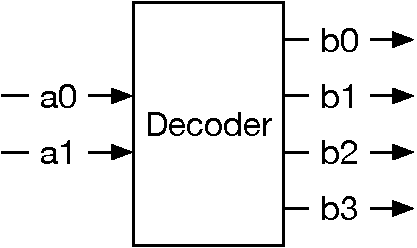
\includegraphics[scale=\scale]{figures/decoder}
  \caption{A 2-bit to 4-bit decoder.}
  \label{fig:decoder}
\end{figure}

Figure~\ref{fig:decoder} shows a 2-bit to 4-bit decoder. We can describe the function
of the decoder with a truth table, such as Table~\ref{tab:decoder}.

\begin{table}
 \centering
 \label{tab:decoder}
  \begin{tabular}{rr}
    \toprule
    a & b \\
    \midrule
    00 & 0001 \\
    01 & 0010 \\
    10 & 0100 \\
    11 & 1000 \\
    \bottomrule 
  \end{tabular} 
  \caption{Truth table for a 2 to 4 decoder.}
\end{table}

A Chisel \code{switch} statement describes the logic as a truth table.
The \code{switch} statement is not part of the core Chisel language.
Therefore, we need to include the elements of the package \code{chisel.util}.

\shortlist{code/encdec_util.txt}

\noindent The following code introduces the \code{switch} statement of Chisel to describe a decoder:

\shortlist{code/encdec_dec.txt}

\noindent The above \code{switch} statement lists all possible values of the \code{sel} signal
and assigns the decoded value to the \code{result} signal.
Note that even if we enumerate all possible input values, Chisel still needs us to assign a
default value, as we do by assigning 0 to \code{result}.
This assignment will never be active and therefore optimized away by the backend tool.
It is intended to avoid situations with incomplete assignments for combinational circuits
(in Chisel a \code{Wire}) that will result in unintended latches in hardware description
languages such as VHDL and Verilog. Chisel does not allow incomplete assignments.

In the example before we used unsigned integers for the signals. Maybe a clearer representation
of an encode circuit uses the binary notation:

\shortlist{code/encdec_decbin.txt}

\todo{from Luca: for very small examples. What if the one-hot input is 256 wires? Can Chisel capture that? Or I need 256 lines? I would suggest to put an additional example. Maybe there is something like the for loop in VHDL.}

A table gives a very readable representation of the decoder function but is also
a little bit verbose.
When examining the table, we see a regular structure: a 1 is shifted left by the number
represented by \code{sel}. Therefore, we can express a decoder with the Chisel shift
operation \code{<<}.

\shortlist{code/encdec_shift.txt}

Decoders are used as a building block for a multiplexer by using the output as an enable
with an AND gate for the multiplexer data input. However, in Chisel, we do not need to construct
a multiplexer, as a \code{Mux} is available in the core library.
Decoders can also be used for address decoding, and then the outputs are used as
select signals, e.g., different IO devices connected to a microprocessor. 


\section{Encoder}

An \myref{https://en.wikipedia.org/wiki/Encoder_(digital)}{encoder}
converts a one-hot encoded input signal into a binary encoded output signal.
The encoder does the inverse operation of a decoder.

\begin{figure}
  \centering
  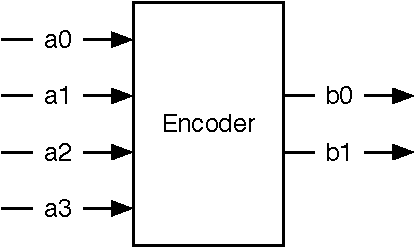
\includegraphics[scale=\scale]{figures/encoder}
  \caption{A 4-bit to 2-bit encoder.}
  \label{fig:encoder}
\end{figure}


\begin{table}
 \centering
 \label{tab:encoder}
  \begin{tabular}{rr}
    \toprule
    a & b \\
    \midrule
    0001 & 00 \\
    0010 & 01 \\
    0100 & 10 \\
    1000 & 11 \\
    ???? & ?? \\
    \bottomrule 
  \end{tabular} 
  \caption{Truth table for a 4 to 2 encoder.}
\end{table}

Figure~\ref{fig:encoder} shows a 4-bit one-hot input to a 2-bit binary output encoder, and
Table~\ref{tab:encoder} shows the truth table of the encode function. However, an encoder
works only as expected when the input signal is one-hot coded. For all other input values, the output
is undefined. As we cannot describe a function with undefined outputs, we use a default
assignment that catches all undefined input patterns.

The following Chisel code assigns a default value of 00 and then uses the switch statement
for the legal input values.

\shortlist{code/encdec_enc.txt}

\section{Exercise}

Describe a combinational circuit to convert a 4-bit binary input to the encoding of a
\myref{https://en.wikipedia.org/wiki/Seven-segment_display}{7-segment display}.
You can either define the codes for the decimal digits, which was the initial
usage of a 7-segment display or additionally, define encodings for the remaining bit pattern
to be able to display all 16 values of a single digit in
\myref{https://en.wikipedia.org/wiki/Hexadecimal}{hexadecimal}.
When you have an FPGA board with a 7-segment display, connect 4 switches or
buttons to the input of your circuit and the output to the 7-segment display.

\chapter{Sequential Building Blocks}

Sequential circuits are circuits where the output depends on the input \emph{and}
previous values. As we are interested in synchronous design (clocked designs),
we mean synchronous sequential circuits when we talk about sequential
circuits.\footnote{We can also build sequential circuits with asynchronous logic and
feedback, but this is a specific niche topic and cannot be expressed in Chisel.}
To build sequential circuits, we need elements that can store state:
the so-called registers.

\section{Registers}

\begin{figure}
  \centering
  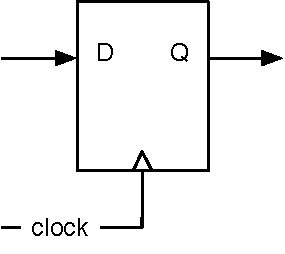
\includegraphics[scale=\scale]{figures/register}
  \caption{A D flip-flop based register.}
  \label{fig:register}
\end{figure}

The fundamental elements for building sequential circuits are registers. A register is a collection
of \myref{https://en.wikipedia.org/wiki/Flip-flop_(electronics)\#D_flip-flop}{D flip-flops}.
A D flip-flop captures the value of its input at the rising edge of the clock and stores
it at its output. Alternatively, in other words: the register updates its output with the value of the input on the rising edge of the clock.

Figure~\ref{fig:register} shows the schematic symbol of a register. It contains an input
\code{D} and an output \code{Q}. Each register also contains an input for a \code{clock} signal.
As this global clock signal is connected to all registers in a synchronous circuit, it is usually
not drawn in the schematic. The little triangle on the bottom of the box symbolizes the
clock input and tells us that this is a register. We omit the clock signal in the following
drawings.
The omission of the global clock signal is also reflected by Chisel where no explicit
connection of a signal to the register's clock input is needed.

In Chisel a register with input \code{d} and output \code{q} is defined with:

\shortlist{code/sequ_reg.txt}

\noindent Note that we do not need to connect a clock to the register, Chisel implicitly does this.
A register's input and output can be arbitrary complex types
made out of a combination of vectors and bundles.

A register can also be defined and used in two steps:

\shortlist{code/sequ_reg2.txt}

First, we define the register and give it a name. Second, we connect the signal
\code{delayIn} to the input of the register. Note also that the name of the register
contains the string \code{Reg}. To easily distinguish between combinational
circuits and sequential circuits, it is common practice to have the marker
\code{Reg} as part of to the name. Also, note that names in Scala (and therefore
also in Chisel) are usually in
\myref{https://en.wikipedia.org/wiki/Camel_case}{CamelCase}.
Variable names start with lowercase and classes start with upper case.

A register can also be initialized on reset. The \code{reset} signal is, as the \code{clock} signal,
implicit in Chisel. We supply the reset value, e.g., zero, as a parameter to the register
constructor \code{RegInit}. The input for the register is connected with a Chisel
assignment statement.

\shortlist{code/sequ_reg_init.txt}

The default implementation of reset in Chisel is a synchronous
reset.\footnote{Support for asynchronous reset is currently under development}
For a synchronous reset no change is needed on a D flip-flop, just a multiplexer
needs to be added to the input that selects between the initialization value under
reset and the data values.


\begin{figure}
  \centering
  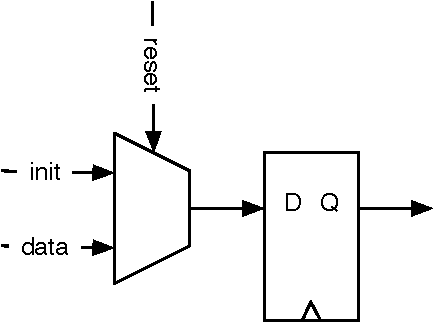
\includegraphics[scale=\scale]{figures/register-reset}
  \caption{A D flip-flop based register with a synchronous reset.}
  \label{fig:register-reset}
\end{figure}

Figure~\ref{fig:register-reset} shows the schematics of a register with a synchronous reset
where the reset drives the multiplexer. However, as synchronous reset is used quite often
modern FPGAs flip-flops contain a synchronous reset (and set) input to not wast LUT
resources for the multiplexer.

Sequential circuits change their value over time. Therefore, their behavior can be described
by a diagram showing the signals over time. Such a diagram is called a waveform or
\myref{https://en.wikipedia.org/wiki/Digital_timing_diagram}{timing diagram}.

\todo{from Luca: Do readers know about timing diagrams?}

\begin{figure}
  \centering
  \includegraphics[scale=1]{figures/reg_wave}
  \caption{A waveform diagram for a register with a reset.}
  \label{fig:register-wave}
\end{figure}

Figure~\ref{fig:register-wave} shows a waveform for the register with a reset
and some input data applied to it.
Time advances from left to right. On top of the figure, we see the clock that drives our circuit.
In the first clock cycle, before a reset, the register is undefined. In the second clock cycle reset
is asserted high, and on the rising edge of this clock cycle (labeled B) the register
captures the initial value of \code{0}. Input \code{inVal} is ignored. In the next clock cycle
\code{reset} is \code{0}, and the value of \code{inVal} is captured on the next rising
edge (labeled C). From then on \code{reset} stays \code{0}, as it should be, and the
register output follows the input signal with one clock cycle delay.

Waveforms are an excellent tool to specify the behavior of a circuit graphically.
Especially in more complex circuits where many operations happen in parallel
and data move pipelined through the circuit, timing diagrams are convenient.
Chisel testers can also produce waveforms during testing that can be displayed
with a waveform viewer and used for debugging.

A typical design pattern is a register with an enable signal. Only when the enable signal
is \code{true} (high), the register captures the input; otherwise, it keeps its old value.
The enable can be implemented, similar to the synchronous reset, with
a multiplexer at the input of the register. One input to the multiplexer is the feedback of the
output of the register.

\begin{figure}
  \centering
  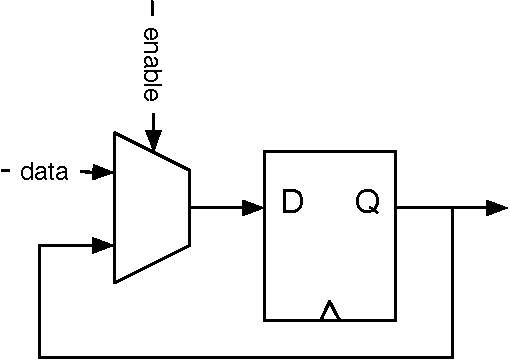
\includegraphics[scale=\scale]{figures/register-enable}
  \caption{A D flip-flop based register with an enable signal.}
  \label{fig:register-enable}
\end{figure}

Figure~\ref{fig:register-enable} shows the schematics of a register with enable.
As this is also a common design pattern, modern FPGA flip-flops contain a
dedicated enable input, and no additional resources are needed.

\begin{figure}
  \centering
  \includegraphics[scale=1]{figures/reg_en_wave}
  \caption{A waveform diagram for a register with an enable signal.}
  \label{fig:register-en-wave}
\end{figure}

Figure~\ref{fig:register-en-wave} shows an example waveform for a register
with enable. Most of the time, enable it high (\code{true}) and the register
follows the input with one clock cycle delay. Only in the fourth clock cycle
\code{enable} is low, and the register keeps its value (5) at rising edge D.

A register with an enable can be described in a few lines of Chisel code
with a conditional update:

\shortlist{code/sequ_reg_ena.txt}

\noindent A register with enable can also be reset:

\shortlist{code/sequ_reg_init_ena.txt}

A register can also be part of an expression. Following circuit detects the rising edge
of a signal by comparing its current value with the one from the last clock cycle.

\shortlist{code/sequ_reg_rising.txt}

Now that we have explored all basic uses of a register, we put those registers to
good use and build more interesting sequential circuits.

\section{Counters}
\label{sec:counter}

\begin{figure}
  \centering
  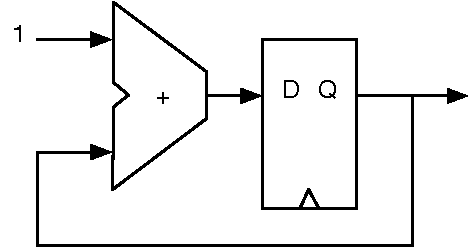
\includegraphics[scale=\scale]{figures/counter}
  \caption{An adder and a register result in counter.}
  \label{fig:counter}
\end{figure}

One of the most basic sequential circuits is a counter. In its simplest form, a counter is a register
where the output is connected to an adder and the adder's output is connected to the input
of the register. Figure~\ref{fig:counter} shows such a free-running counter.

A free-running counter with a 4-bit register counts from 0 to 15 and then wraps around
to 0 again. A counter shall also be reset to a known value.

\shortlist{code/sequ_free_counter.txt}

\noindent When we want to count events, we use a condition to  increment the counter.

\shortlist{code/sequ_event_counter.txt}

\subsection{Counting Up and Down}

To count up to a value and then restart with \code{0}, we need to compare
the counter value with a maximum constant, e.g., with a \code{when}
conditional statement.

\shortlist{code/when_counter.txt}

\noindent We can also use a multiplexer for our counter:

\shortlist{code/mux_counter.txt}

\noindent If we are in the mood of counting down, we start (reset the counter register)
with the maximum value and reset the counter to that value when reaching 0.

\shortlist{code/down_counter.txt}

\noindent As we are writing and using more counters, we can
define a function with a parameter to generate a counter for us.

\shortlist{code/function_counter.txt}

\noindent The last statement of the function \code{genCounter} is the return
value of the function, in this example, the counting register \code{cntReg}.

Note, that in all the examples our counter had values between \code{0} and
\code{N}, including \code{N}. If we want to count 10 clock cycles we need
to set \code{N} to 9. Setting \code{N} to 10 would be a classic example of an
\myref{https://en.wikipedia.org/wiki/Off-by-one_error}{off-by-one error}.

\subsection{Generating Timing with Counters}

Besides counting events, counters are often used to generate timing.
A synchronous circuit runs with a clock with a fixed frequency.
The circuit proceeds in those clock ticks. There is no notion of time in a digital
circuit other than counting clock ticks. If we know the clock frequency, we
can generate circuits that generate timed events, such as blinking a LED
at some frequency as we have shown in the Chisel ``Hello World'' example.

A common practice is to generate single-cycle \emph{ticks} with a frequency $f_{tick}$
that we need in our circuit. That tick occurs every $n$ clock cycles,
where $n = f_{clock}/f_{tick}$ and the tick is precisely one clock cycle long.
This tick is \emph{not} used as a derived clock, but as an enable signal for
registers in the circuit that shall logically operate at frequency $f_{tick}$.
Figure~\ref{fig:tick-wave} shows an example of a tick generated every
3 clock cycles.

\begin{figure}
  \centering
  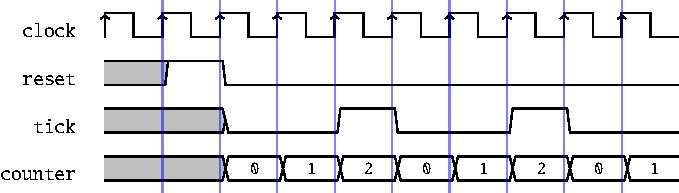
\includegraphics[scale=1]{figures/tick_wave}
  \caption{A waveform diagram for the generation of a slow frequency tick.}
  \label{fig:tick-wave}
\end{figure}


In the following circuit, we describe a counter that counts from \code{0}
to the maximum value of \code{N - 1}. When the maximum value is reached,
the \code{tick} is \code{true} for a single cycle, and the counter is reset to \code{0}.
When we count from \code{0} to \code{N - 1}, we generate one logical tick
every \code{N} clock cycles.

\shortlist{code/sequ_tick_gen.txt}

\noindent This logical timing of one tick every $n$ clock cycles can then be used
to advance other parts of our circuit with this slower, logical clock.
In the following code, we use just another counter that increments by \code{1}
every $n$ clock cycles.

\shortlist{code/sequ_tick_counter.txt}

Examples of the usage of this slower \emph{logical} clock are: blinking an LED,
generating the baud rate for a serial bus, generating signals for 7-segment
display multiplexing, and subsampling input values for debouncing of buttons
and switches. 

Although width inference should size the registers, it is better to explicitly
specify the width with the type at register definition or with the
initialization value. Explicit width definition can avoid surprises when a reset value of \code{0.U}
results in a counter with a width of a single bit.

\subsection{The Nerd Counter}

Many of us feel like being a \myref{https://en.wikipedia.org/wiki/Nerd}{nerd}, sometimes.
For example, we want to design a highly optimized version of our counter/tick generation.
A standard counter needs following resources: one register, one adder (or subtractor),
and a comparator. We cannot do much about the register or the adder. If we count
up, we need to compare against a number, which is a bit string. The comparator
can be built out of inverters for the zeros in the bit string and a large AND gate.
When counting down to zero, the comparator is a large NOR gate, which might be
a little bit cheaper than the comparator against a constant in an ASIC.
In an FPGA ,where logic is built out of lookup tables, there is no difference between comparing
against a 0 or 1 bit. The resource requirement is the same for the up and down counter.

However, there is still one more trick a clever hardware designer can pull off.
Counting up or down needed a comparison against all counting bits, so far.
What if we count from N-2 down to -1? A negative number has the most significant bit
set to 1, and a positive number has this bit set to 0. We need to check this bit only to detect
that our counter reached -1. Here it is, the counter created by a nerd:

\shortlist{code/nerd_counter.txt}

\section{Memory}

A memory can be built out of a collection of registers, in Chisel a \code{Reg} of a \code{Vec}.
However, this is expensive in hardware, and larger memory structures are built
as \myref{https://en.wikipedia.org/wiki/Static_random-access_memory}{SRAM}.
For an ASIC, a memory compiler constructs memories.
FPGAs contain on-chip memory blocks, also called block RAMs.
Those on-chip memory blocks can be combined for larger memories.
Memories in an FPGA usually have one read and one write port, or
two ports where the direction can be switched.

FPGAs (and also ASICs) usually support synchronous memories.
Synchronous memories have registers on their inputs (read and write address, write data,
and write enable). That means the read data is available one clock
cycle after setting the address.

\begin{figure}
  \centering
  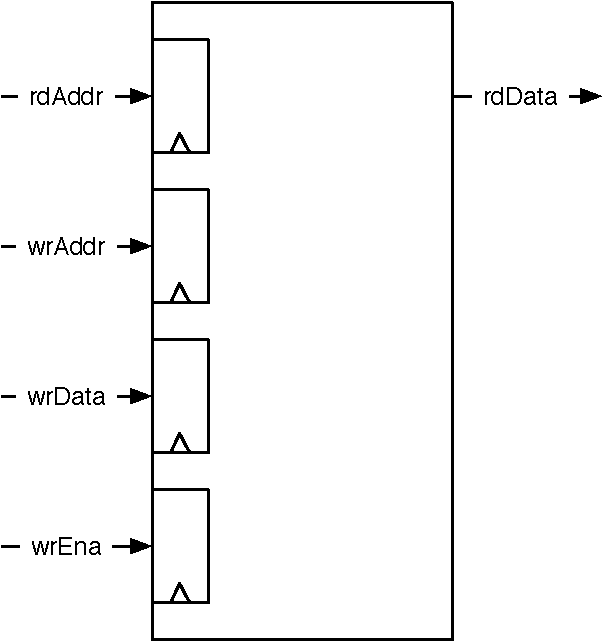
\includegraphics[scale=\scale]{figures/memory}
  \caption{A synchronous memory.}
  \label{fig:memory}
\end{figure}

Figure~\ref{fig:memory} shows the schematics of such a synchronous memory.
The memory is dual-ported with one read port and one write port.
The read port has a single input, the read address (\code{rdAddr}) and
one output, the read data (\code{rdData}).
The write port has three inputs: the address (\code{wrAddr}), the data
to be written (\code{wrData}), and a write enable (\code{wrEna}).
Note that for all inputs, there is a register within the memory showing the
synchronous behavior.

To support on-chip memory, Chisel provides the memory constructor \code{SyncReadMem}.
Listing~\ref{lst:memory} shows a component \code{Memory} that implements
1~KB of memory with byte-wide input and output data and a write enable.

\longlist{code/memory.txt}{1 KB of synchronous memory.}{lst:memory}

An interesting question is which value is returned from a read when in the same clock
cycle a new value is written the same address that is read out.
We are interested in the read-during-write behavior of the memory.
There are three possibilities: the newly written value, the old value, or undefined
(which might be a mix of some bits from the old value and some of the newly written data).
Which possibility is available in an FPGA depends on the FPGA type and
sometimes can be specified.
Chisel documents that the read data is undefined.

\begin{figure}
  \centering
  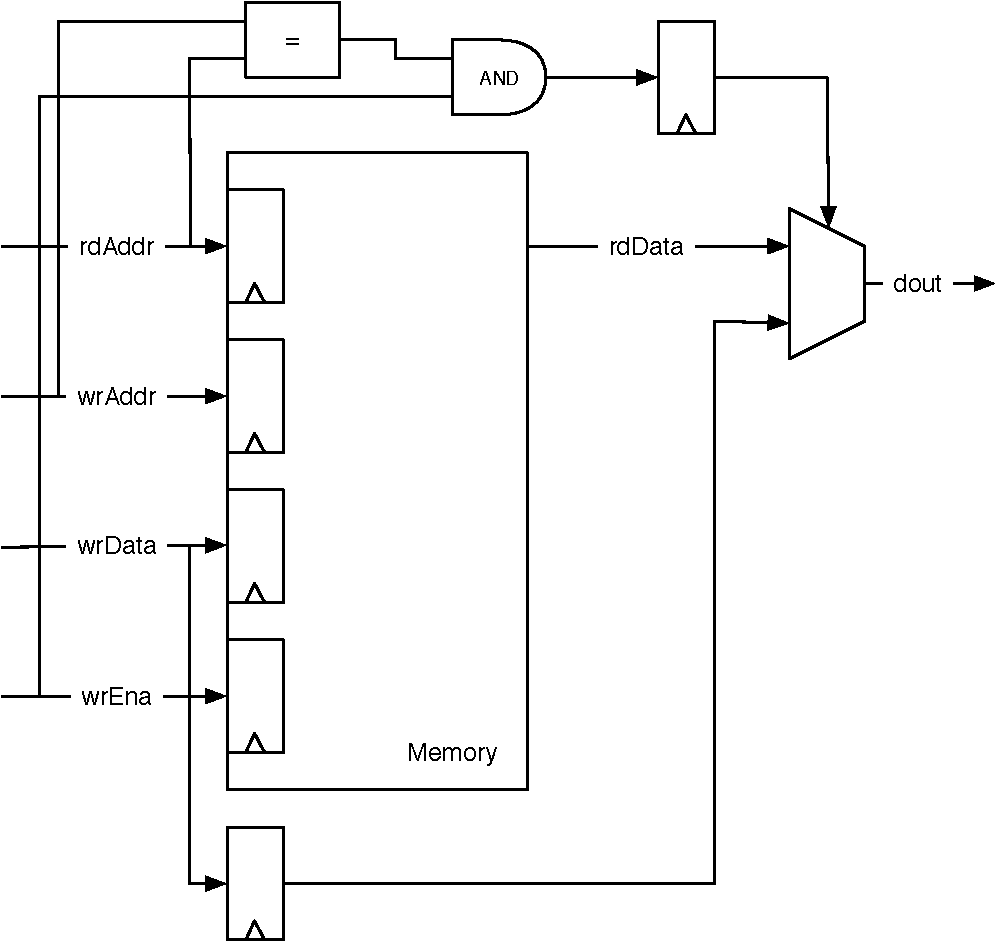
\includegraphics[scale=\scale]{figures/memory-forwarding}
  \caption{A synchronous memory with forwarding for a defined read-during-write behavior.}
  \label{fig:memory:forwarding}
\end{figure}

If we want to read out the newly written value, we can build a forwarding
circuit that detects that the addresses are equal and \emph{forwards} the
write data. Figure~\ref{fig:memory:forwarding} shows the memory with
the forwarding circuit. Read and write addresses are compared and gated with
the write enable to select between the forwarding path of the write data or the
memory read data. The write data is delayed by one clock cycle with a register.

Listing~\ref{lst:memory:forward} shows the Chisel code for a synchronous memory
including the forwarding circuit. We need to store the write data into a register
(\code{wrDataReg}) to be available in the next clock cycle the synchronous
memory also has a one clock cycle latency.
We compare the two input addresses (\code{wrAddr} and \code{rdAddr})
and check if \code{wrEna} is true for the forwarding condition.
That condition is also delayed by one clock cycle.
A multiplexer selects between the forwarding (write) data or the read
data from memory.

\longlist{code/memory_forwarding.txt}{A memory with a forwarding circuit.}{lst:memory:forward}



Chisel also provides \code{Mem}, which represents a memory with synchronous
write and an asynchronous read. As this memory type is usually not directly available
in an FPGA, the synthesize tool will build it out of flip-flops.
Therefore, we recommend using \code{SyncReadMem}.


\section{Exercise}

Use the 7-segment encoder from the last exercise and add a 4-bit counter as input
to switch the display from \code{0} to \code{F}. When you directly connect this
counter to the clock of the FPGA board, you will see all 16 numbers
overlapped (all 7 segments will light up).
Therefore, you need to slow down the counting. Create a second
counter that can generate a single-cycle \emph{tick} signal every 500 milliseconds.
Use that signal as enable signal for the 4-bit counter.

\todo{Luca: More exercises would be nice. Maybe in the future?}

\chapter{Finite-State Machines}

A finite-state machine (FSM) is a basic building block in digital design.
An FSM can be described as a set of \emph{states} and conditional (guarded)
\emph{state transitions} between states. 
An FSM has an initial state, which is set on reset.
FSMs are also called synchronous sequential circuits.

An implementation of an FSM consists of three parts: (1) a register that holds the current state,
(2) combinational logic that computes the next state that depends on the current
state and the input, and (3) combinational logic that computes the output of the FSM.

In principle, every digital circuit that contains a register or other memory elements
to store state can be described as a single FSM. However, this might
not be practical, e.g., try to describe your laptop as a single FSM.
In the next chapter, we describe how to build larger systems
out of smaller FSMs by combining them into communicating FSMs.

\section{Basic Finite-State Machine}

\begin{figure}
  \centering
  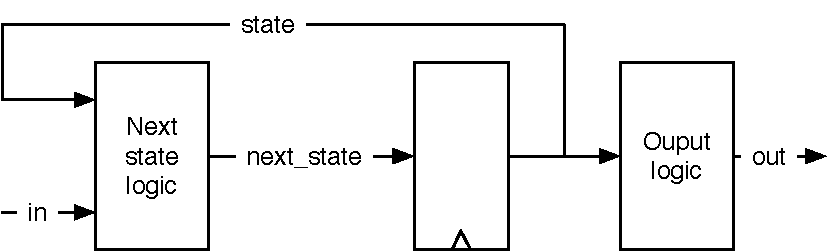
\includegraphics[scale=\scale]{figures/fsm}
  \caption{A finite state machine (Moore type).}
  \label{fig:fsm}
\end{figure}

Figure~\ref{fig:fsm} shows the schematics of an FSM. The register contains the current \code{state}.
The next state logic computes the next state value (\code{next\_state})
from the current \code{state} and the input (\code{in}).
On the next clock tick, \code{state} becomes \code{next\_state}.
The output logic computes the output (\code{out}). As the output depends on the current
state only, this state machine is called a
\myref{https://en.wikipedia.org/wiki/Moore_machine}{Moore machine}.

A \myref{https://en.wikipedia.org/wiki/State_diagram}{state diagram}
describes the behavior of such an FSM visually.
In a state diagram, individual states are depicted as circles labeled
with the state names.
State transitions are shown with arrows between states.
The guard (or condition) when this transition is taken is drawn as a label
for the arrow.

Figure~\ref{fig:diag-moore} shows the state diagram of a simple example FSM.
The FSM has three states: \emph{green}, \emph{orange}, and \emph{red},
indicating a level of alarm. The FSM starts at the \emph{green} level.
When a \emph{bad event} happens the alarm level is switched to \emph{orange}.
On a second bad event, the alarm level is switched to \emph{red}.
In that case, we want to ring a bell; \emph{ring bell} it the only output of this FSM.
We add the output to the \emph{red} state.
The alarm can be reset with a \emph{clear} signal.

\begin{figure}
  \centering
  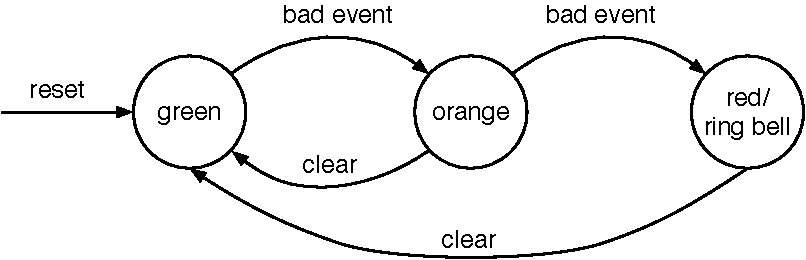
\includegraphics[scale=\scale]{figures/state-diag-moore}
  \caption{The state diagram of an alarm FSM.}
  \label{fig:diag-moore}
\end{figure}

Although a state diagram may be visually pleasing and the function of an FSM
can be grasped quickly, a state table may be quicker to write down.
Table~\ref{tab:state:table} shows the state table for our alarm FSM.
We list the current state, the input values, the resulting next state, and
the output value for the current state. In principle, we would need to
specify all possible inputs for all possible states. This table would have
$3 \times 4 = 12$ rows. We simplify the table by indicating that the \emph{clear}
input is a don't care when a \emph{bad event} happens. That means
\emph{bad event} has priority over \emph{clear}. The output column
has some repetition. If we have a larger FSM and/or more outputs, we
can split the table into two, one for the next state logic and one for the
output logic.

\begin{table}
\centering
\caption{State table for the alarm FSM.}
\begin{tabular}{ccccc}
\toprule
& \multicolumn{2}{c}{Input} \\
\cmidrule{2-3}
State &  Bad event & Clear & Next state & Ring bell \\
\midrule
green & 0 & 0 & green & 0 \\
green & 1 & - & orange & 0 \\
orange & 0 & 0 & orange & 0 \\
orange & 1 & - & red & 0 \\
orange & 0 & 1 & green & 0 \\
red & 0 & 0 & red & 1 \\
red & 0 & 1 & green & 1 \\
\bottomrule
\end{tabular}
\label{tab:state:table}
\end{table}

Finally, after all the design of our warning level FSM, we shall code it in Chisel.
Listing~\ref{lst:fsm:alarm} shows the Chisel code for the alarm FSM.
Note, that we use the Chisel type \code{Bool} for the inputs and the
output of the FSM.
To use \code{Enum} and the \code{switch} control instruction, we need to
import \code{chisel3.util.\_}.

\longlist{code/simple_fsm.txt}{The Chisel code for the alarm FSM.}{lst:fsm:alarm}

The complete Chisel code for this simple FSM fits into one page.
Let us step through the individual parts.
The FSM has two input and a single output signal, captured in a Chisel \code{Bundle}:
%
\shortlist{code/simple_fsm_io.txt}


\noindent Quite some work has been spent in optimal state encoding. Two common options
are binary or one-hot encoding. However, we leave those low-level decisions to
the synthesize tool and aim for readable code.\footnote{In the current version
of Chisel the \code{Enum} type represents states in binary encoding.
If we want a different encoding, e.g., one-hot encoding, we can define Chisel
constants for the state names.}
Therefore, we use an enumeration type with symbolic names for the states:

\shortlist{code/simple_fsm_states.txt}

\noindent The individual state values are described as a list where the individual
elements are concatenated with the \code{::} operator; \code{Nil} represents
the end of the list. An \code{Enum} instance is \emph{assigned} to the list of states.
The register holding the state is defined with the \emph{green} state as the reset value:

\shortlist{code/simple_fsm_register.txt}

\noindent The meat of the FSM is in the next state logic. We use a Chisel switch on the
state register to cover all states. Within each \code{is} branch we code the next state
logic, which depends on the inputs, by assigning a new value for our state register:

\shortlist{code/simple_fsm_next.txt}

\noindent Last, but not least, we code our \emph{ringing bell} output to be true when
the state is \emph{red}.

\shortlist{code/simple_fsm_output.txt}

Note that we did \emph{not} introduce a \code{next\_state} signal for the register input,
as it is common practice in Verilog or VHDL.
Registers in Verilog and VHDL are described in a special syntax and cannot
be assigned (and reassigned) within a combinational block.
Therefore, the additional signal, computed in a combinational block, is
introduced and connected to the register input.
In Chisel a register is a base type and can be freely used within a combinational block.

\section{Faster Output with a Mealy FSM}

On a Moore FSM, the output depends only on the current state.
That means that a change of an input can be seen as a change of the
output \emph{earliest} in the next clock cycle.
If we want to observe an immediate change, we need a combinational
path from the input to the output.
Let us consider a minimal example, an edge detection circuit.
We have seen this Chisel one-liner before:

\shortlist{code/sequ_reg_rising.txt}

\begin{figure}
  \centering
  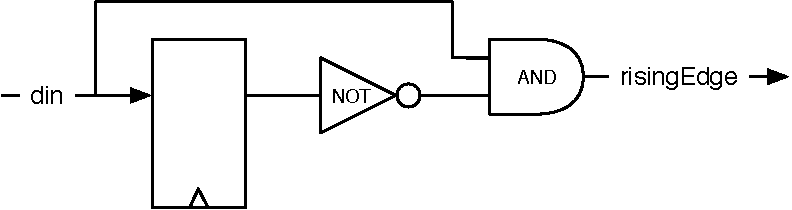
\includegraphics[scale=\scale]{figures/fsm-rising}
  \caption{A rising edge detector (Mealy type FSM).}
  \label{fig:rising}
\end{figure}

Figure~\ref{fig:rising} shows the schematic of the rising edge detector.
The output becomes 1 for one clock cycle when the current input is 1
and the input in the last clock cycle was 0.
The state register is just a single D flip-flop where the next state
is just the input. We can also consider this as a delay element of one
clock cycle. The output logic \emph{compares} the current
input with the current state.



When the output depends also on the input, i.e., there is a combinational path between
the input of the FSM and the output, this is called a
\myref{https://en.wikipedia.org/wiki/Mealy_machine}{Mealy machine}.

\begin{figure}
  \centering
  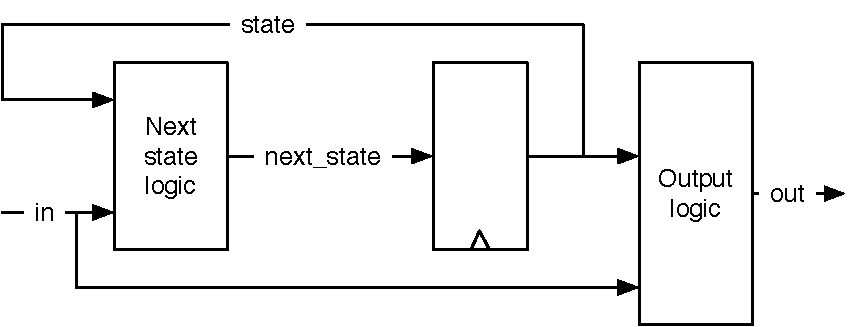
\includegraphics[scale=\scale]{figures/mealy}
  \caption{A Mealy type finite state machine.}
  \label{fig:mealy}
\end{figure}

Figure~\ref{fig:mealy} shows the schematic of a Mealy type FSM.
Similar to the Moore FSM, the register contains the current \code{state}, and
the next state logic computes the next state value (\code{next\_state})
from the current \code{state} and the input (\code{in}).
On the next clock tick, \code{state} becomes \code{next\_state}.
The output logic computes the output (\code{out}) from the current state
\emph{and} the input to the FSM.


\begin{figure}
  \centering
  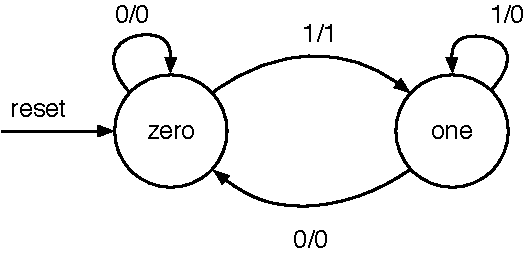
\includegraphics[scale=\scale]{figures/state-diag-mealy}
  \caption{The state diagram of the rising edge detector as Mealy FSM.}
  \label{fig:diag:mealy}
\end{figure}

Figure~\ref{fig:diag:mealy} shows the state diagram of the Mealy FSM for the
edge detector. As the state register consists just of a single D flip-flop,
only two states are possible, which we name \code{zero} and \code{one} in this
example.
As the output of a Mealy FSM does not only depend on the state, but also
on the input, we cannot describe the output as part of the state circle.
Instead, the transitions between the states are labeled with the input
value (condition) \emph{and} the output (after the slash).
Note also that we draw self transitions, e.g., in state \code{zero} when
the input is \code{0} the FSM stays in state \code{zero}, and the output is {0}.
The rising edge FSM generates the \code{1} output only on the transition
from state \code{zero} to state \code{one}. In state \code{one}, which represents
that the input is now \code{1}, the output is \code{0}. We only want a single (cycle)
puls for each rising edge of the input.

\longlist{code/rising_fsm.txt}{Rising edge detection with a Mealy FSM.}{lst:fsm:rising}

Listing~\ref{lst:fsm:rising} shows the Chisel code for the rising edge detection
with a Mealy machine.
As in the previous example, we use the Chisel type \code{Bool} for the
single-bit input and output.
The output logic is now part of the next state logic; on the transition from
\code{zero} to \code{one}, the output is set to \code{true.B}. Otherwise,
the default assignment to the output (\code{false.B}) counts.

One can ask if a full-blown FSM is the best solution for the edge detection circuit,
especially, as we have seen a Chisel one-liner for the same functionality.
The hardware consumptions is similar. Both solutions need a single D flip-flop
for the state. The combinational logic for the FSM is probably a bit more complicated, as
the state change depends on the current state and the input value.
For this function, the one-liner is easier to write and easier to read,
which is more important. Therefore, the one-liner is the preferred solution.

We have used this example to show one of the smallest possible Mealy FSMs.
FSMs shall be used for more complex circuits with three and more states.

\section{Moore versus Mealy}

To show the difference between a Moore and Mealy FSM, we redo the edge
detection with a Moore FSM. 

\begin{figure}
  \centering
  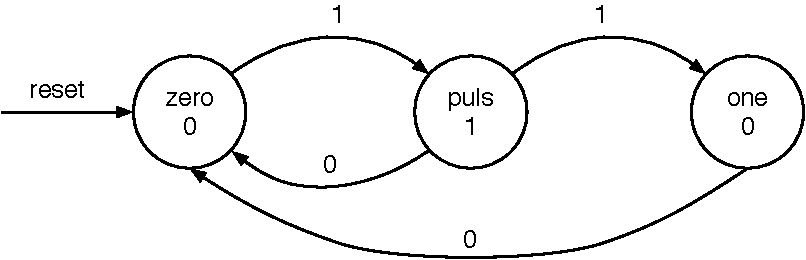
\includegraphics[scale=\scale]{figures/state-diag-rising-moore}
  \caption{The state diagram of the rising edge detector as Moore FSM.}
  \label{fig:diag:rising:moore}
\end{figure}

Figure~\ref{fig:diag:rising:moore} shows the state diagram for the rising
edge detection with a Moore FSM. The first thing to notice is that the Moore FSM
needs three states, compared to two states in the Mealy version.
The state \code{puls} is needed to produce the single-cycle puls.
The FSM stays in state \code{puls} just one clock cycle and then
proceeds either back to the start state \code{zero} or to the \code{one}
state, waiting for the input to become 0 again.
We show the input condition on the state transition arrows and the
FSM output within the state representing circles.

\longlist{code/rising_moore_fsm.txt}{Rising edge detection with a Moore FSM.}{lst:fsm:rising:moore}

Listing~\ref{lst:fsm:rising:moore} shows the Moore version of the rising edge detection
circuit. Is uses double the number of D flip-flops than the Mealy or direct
coded version. The resulting next state logic is therefore also larger
than the Mealy or direct coded version.

\begin{figure}
  \centering
  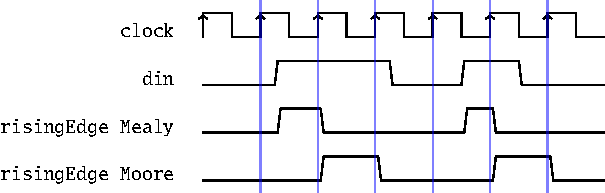
\includegraphics[scale=1]{figures/rising}
  \caption{Mealy and a  Moore FSM waveform for rising edge detection.}
  \label{fig:rising}
\end{figure}

Figure~\ref{fig:rising} shows the waveform of a Mealy and a  Moore version
of the rising edge detection FSM. We can see that the Mealy output closely
follows the input rising edge, while the Moore output rises after the clock tick.
We can also see that the Moore output is one clock cycle wide, where the Mealy
output is usually less than a clock cycle.

From the above example, one is tempted to find Mealy FSMs the \emph{better}
FSMs as they need less state (and therefore logic) and react faster than a Moore FSM.
However, the combinational path within a Mealy machine can cause trouble in
larger designs. First, with a chain of communicating FSM (see next chapter), this
combinational path can become lengthy. Second, if the communicating FSMs build
a circle, the result is a combinational loop, which is an error in synchronous design.
Due to a cut in the combinational path with the state register in a Moore FSM,
all the above issues do not exist for communicating Moore FSMs.

In summary, Moore FSMs combine better for communicating state machines; they
are \emph{more robust} than Mealy FSMs. Use Mealy FSMs only when the reaction within the same
cycle is of utmost importance. Small circuits such as the rising edge detection,
which are practically Mealy machines, are fine as well.

\section{Exercise}

% This is a boring example, maybe I can find something more interesting
In this chapter, you have seen many examples of very small FSMs.
Now it is time to write some \emph{real} FSM code.
Pick a little bit more complex example and implement the FSM and
write a test bench for it.

A classic example for a FSM is a traffic light controller (see~\cite[Section~14.3]{dally:vhdl:2016}).
A traffic light controller has to ensure that on a switch from red to green
there is a phase in between where both roads in the intersection
have a no-go light (red and orange).
To make this example a little bit more interesting, consider a priority road.
The minor road has two car detectors (on both entries into the intersection).
Switch to green for the minor road only when a car is detected and then switch
back to green for the priority road.

\todo{Luca: Greatest common divisor with Euclide algorithm can be also a nice exercise.
Martin: but this is shown at the Chisel homepage without an FSM.}

\chapter{Communicating State Machines}

A problem is often too complex to describe it with a single FSM.
In that case, the problem can be divided into two or more smaller and simpler FSMs.
Those FSMs then communicate with signals. One FSMs output is
another FSMs input, and the FSM watches the output of the other FSM.
When we split a large FSM into simpler ones, this is called factoring FSMs.
However, often communicating FSMs are directly designed from the specification,
as often a single FSM would be infeasible large.

\section{A Light Flasher Example}

To discuss communicating FSMs, we use an example
from~\cite[Chapter~17]{dally:vhdl:2016}, the light flasher.
The light flasher has one input \code{start} and one output
\code{light}. The specification of the light flasher is as follows:
\begin{itemize}
\item when \code{start} is high for one clock cycle, the flashing
sequence starts;
\item the sequence is to flash three times;
\item where the \code{light} goes \emph{on} for six clock cycles, and the \code{light} goes \emph{off} for four clock cycles between flashes;
\item after the sequence, the FSM switches the \code{light} \emph{off} and waits
for the next start.
\end{itemize}

The FSM for a direct implementation\footnote{The state diagram is shown
in~\cite[p.~376]{dally:vhdl:2016}.} has 27 states:
one initial state that is waiting for the input, $3 \times 6$ states for the three
\emph{on} states and $2 \times 4$ states for the \emph{off} states.
We do not show the code for this simple-minded implementation of the light
flasher.

The problem can be solved more elegantly by factoring this large FSM into
two smaller FSMs: the master FSM implements the flashing logic, and the timer FSM
implements the waiting. Figure~\ref{fig:flasher} shows the composition of
the two FSMs.

\begin{figure}
  \centering
  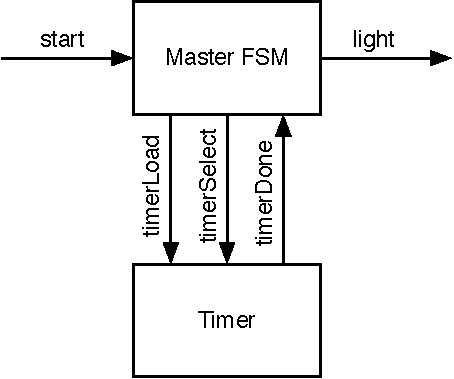
\includegraphics[scale=\scale]{figures/flasher}
  \caption{The light flasher split into a Master FSM and a Timer FSM.}
  \label{fig:flasher}
\end{figure}

The timer FSM counts down for 6 or 4 clock cycles to produce the desired timing.
The timer specification is as follows:

\begin{itemize}
\item when \code{timerLoad} is asserted, the timer loads a value into the down counter,
independent of the state;
\item \code{timerSelect} selects between 5 or 3 for the load;
\item \code{timerDone} is asserted when the counter completed the countdown
and remains asserted;
\item otherwise, the timer counts down.
\end{itemize}

\noindent Following code shows the timer FSM of the light flasher:

\shortlist{code/flasher_timer.txt}

\noindent Listing~\ref{lst:flasher:master} shows the master FSM.

\longlist{code/flasher_fsm.txt}{Master FSM of the light flasher.}{lst:flasher:master}

\begin{figure}
  \centering
  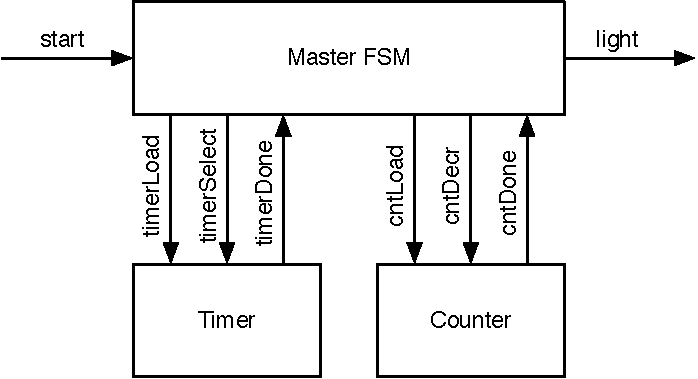
\includegraphics[scale=\scale]{figures/flasher2}
  \caption{The light flasher split into a Master FSM, a Timer FSM, and a Counter FSM.}
  \label{fig:flasher2}
\end{figure}

This solution with a master FSM and a timer has still redundancy in the code
of the master FSM. States \code{flash1}, \code{flash2}, and \code{flash3}
are performing the same function, states \code{space1} and \code{space2} as well.
We can factor out the number of remaining flashes into a second counter.
Then the master FSM is reduced to three states: \code{off}, \code{flash},
and \code{space}.

Figure~\ref{fig:flasher2} shows the design with a master FSM and two FSMs
that count: one FSM to count clock cycles for the interval length of \emph{on}
and \emph{off}; the second FSM to count the remaining flashes.

Following code shows the down counter FSM:

\shortlist{code/flasher2_counter.txt}

\noindent Note, that the counter is loaded with 2 for 3 flashes, as it counts the
\emph{remaining} flashes and is decremented in state \code{space} when the timer
is done. Listing~\ref{lst:flasher2:master} shows the master FSM for the double refactored flasher.

\longlist{code/flasher2_fsm.txt}{Master FSM of the double refactored light flasher.}{lst:flasher2:master}

Besides having a master FSM that is reduced to just three states, our current solution
is also better configurable. No FSM needs to be changed if we want to change
the length of the \emph{on} or \emph{off} intervals or the number of flashes.

In this section, we have explored communicating circuits, especially FSM, that
only exchange control signals. However, circuits can also exchange data.
For the coordinated exchange of data, we use handshake signals.
The next section describes the ready-valid interface for flow control of
unidirectional data exchange.

\section{State Machine with Datapath}

One typical example of communicating state machines is a state machine
combined with a datapath. This combination is often called a finite state machine
with datapath (FSMD). The state machine controls the datapath, and the datapath
performs the computation. The FSM input is the input from the environment and the input
from the datapath. The data from the environment is fed into the datapath, and the
data output comes from the datapath. Figure~\ref{fig:popcnt-fsmd} shows an example
of the combination of the FSM with the datapath.

\begin{figure}
  \centering
  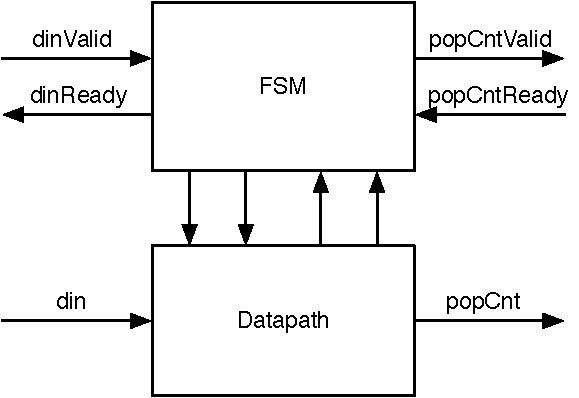
\includegraphics[scale=\scale]{figures/popcnt-fsmd}
  \caption{A state machine with a datapath.}
  \label{fig:popcnt-fsmd}
\end{figure}

\subsection{Popcount Example}

The FSMD shown in Figure~\ref{fig:popcnt-fsmd} serves as an example that computes the
popcount, also called the \myref{https://en.wikipedia.org/wiki/Hamming_weight}{Hamming weight}.
The Hamming weight is the number of symbols different from the zero symbol.
For a binary string, this is the number of `1's.

The popcount unit contains the data input \code{din} and the result output \code{popCount},
both connected to the datapath. For the input and the output we use a ready-valid handshake.
When data is available, valid is asserted. When a receiver can accept data it asserts ready.
When both signals are asserted the transfer takes place. The handshake signals are connected
to the FSM. The FSM is connected with the datapath with control signals towards the datapath
and with status signals from the datapath.

\begin{figure}
  \centering
  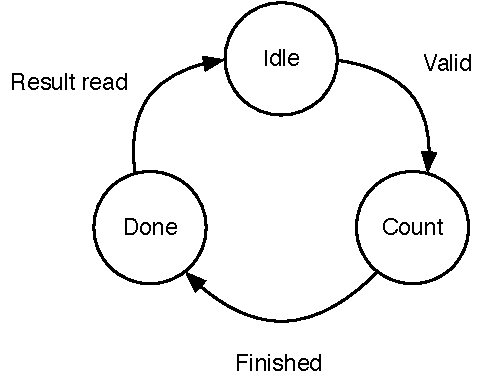
\includegraphics[scale=\scale]{figures/popcnt-states}
  \caption{State diagram for the popcount FSM.}
  \label{fig:popcnt-states}
\end{figure}

As a next step, we can design the FSM, starting with a state diagram, shown in
Figure~\ref{fig:popcnt-states}. We start in state \code{Idle}, where the FSM waits
for input. When data arrives, signaled with a valid signal, the FSM advances to state \code{Load}
to load a shift register. The FSM proceeds to the next state \code{Count}, there the number
of `1's is counted sequentially. We use a shift register, an adder, an accumulator
register, and a down counter to perform the computation. When the down counter reaches
zero, we are finished and the FSM moves to state \code{Done}. There the FSM signals with a valid
signal that the popcount value is ready to be consumed. On a ready signal from the
receiver, the FSM moves back to the \code{Idle} state, ready to compute the next popcount.

The top level component, shown in Listing~\ref{lst:pop:top} instantiates the FSM and the datapath components and connects
them with bulk connections.

\longlist{code/popcnt_main.txt}{The top level of the popcount circuit.
\todo{Bulk connection should be used here (and tested).}}{lst:pop:top}

\begin{figure}
  \centering
  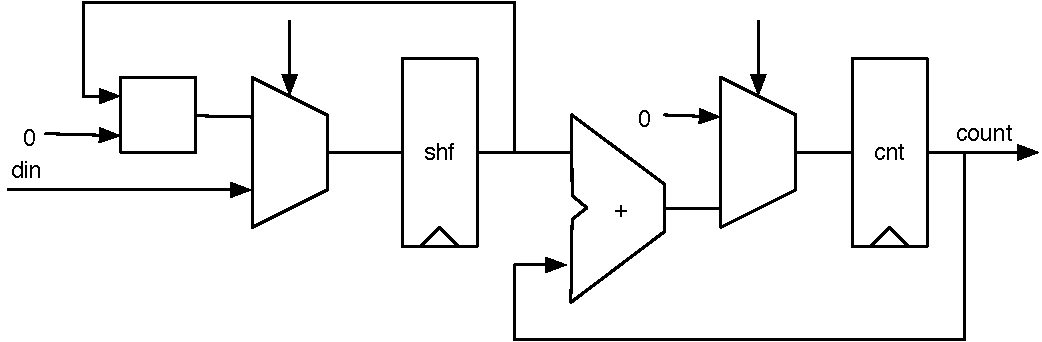
\includegraphics[scale=\scale]{figures/popcnt-data}
  \caption{Datapath for the popcount circuit.}
  \label{fig:popcnt-data}
\end{figure}

Figure~\ref{fig:popcnt-data} shows the datapath for the popcount circuit.
The data is loaded into the \code{shf} register. On the load also the \code{cnt}
register is reset to 0. To count the number of `1's, the \code{shf} register is shifted
right, and the least significant bit is added to \code{cnt} each clock cycle.
A counter, not shown in the figure, counts down until all bits have been shifted
through the least significant bit. When the counter reaches zero, the popcount
has finished. The FSM switches to state \code{Done} and signals the result
by asserting \code{popCntReady}. When the result is read, signaled by asserting
\code{popCntValid} the FSW switches back to \code{Idle}.

On a \code{load} signal, the \code{regData} register is loaded with the input,
the \code{regPopCount} register reset to 0, and the counter register \code{regCount}
set to the number of shifts to be performed.

Otherwise, the \code{regData} register is shifted to the right, the least significant bit
of the \code{regData} register added to the \code{regPopCount} register, and the counter
decremented until it is 0. When the counter is 0, the output contains the popcount.
Listing~\ref{lst:pop:data} shows the Chisel code for the datapath of the popcount
circuit.

\longlist{code/popcnt_data.txt}{Datapath of the popcount circuit.}{lst:pop:data}

The FSM starts in state \code{idle}. On a valid signal for the input data (\code{dinValid}) it
switches to the \code{count} state and waits till the datapath has finished counting.
When the popcount is valid, the FSM switches to state \code{done} and waits till the
popcount is read (signaled by \code{popCntReady}).
Listing~\ref{lst:pop:fsm} shows the code of the FSM.

\longlist{code/popcnt_fsm.txt}{The FSM of the popcount circuit.}{lst:pop:fsm}

\section{Ready-Valid Interface}

\todo{Luca: This comes very sudden after all this FSM reading.
Maybe give some more context and a timing diagram.}

Communication of subsystems can be generalized to the movement
of data and handshaking for flow control. In the popcount example,
we have seen a handshaking interface for the input and the output data
using valid and ready signals.

\begin{figure}
  \centering
  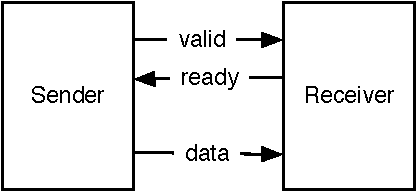
\includegraphics[scale=\scale]{figures/readyvalid}
  \caption{The ready-valid flow control.}
  \label{fig:readyvalid}
\end{figure}

The ready-valid interface~\cite[p.~480]{dally:vhdl:2016} is a simple flow
control interface consisting of \code{data} and a \code{valid} signal at the
sender side and a \code{ready} signal at the receiver side (see
Figure~\ref{fig:readyvalid}). The sender asserts \code{valid} when \code{data} is available,
and the receiver asserts \code{ready} when it is ready to receive one word
of data. The transmission of the data happens when both signals, \code{valid}
and \code{ready}, are asserted. If either of the two signals is not asserted,
no transfer takes place.

To make this interface composable neither \code{ready} not \code{valid} is
allowed to depend combinational on the other signal.

\todo{Read and cite AXI}

\chapter{Hardware Generators}

The strength of Chisel is that it allows us to write so-called hardware generators.
With older hardware description languages, such as VHDL and Verilog,
we usually use another language, e.g., Java or Python, to generate hardware.
The author has often written small Java programs to generate VHDL tables.
In Chisel, the full power of Scala (and Java libraries) is available at hardware
construction. Therefore, we can write our hardware generators in the same
language and execute them as part of the Chisel circuit generation.

\section{Configure with Parameters}

Chisel components and functions can be configured with parameters.
Parameters can be as simple as an integer constant, but can also be a Chisel
hardware type.

\subsection{Simple Parameters}

The basic way to parameterize a circuit is to define a bit width as a parameter.
Parameters can be passed as arguments to
the constructor of the Chisel module. Following example is a toy example of
a module that implements an adder with a configurable bit width.
The bit width \code{n} is a parameter (of Scala type \code{Int}) of the component
passed into the constructor that can be used in the IO bundle.

\shortlist{code/param_adder.txt}

\noindent Parameterized versions of the adder can be created as follows:

\shortlist{code/use_param_adder.txt}

\subsection{Functions with Type Parameters}

Having the bit width as a configuration parameter is just the starting point for
hardware generators. A very flexible configuration is the usage of types.
That feature allows for Chisel to provide a multiplexer (\code{Mux}) that
can accept any types for the multiplexing.
To show how to use types for the configuration, we build a multiplexer
that accepts arbitrary types. Following function defines the multiplexer:

\shortlist{code/param_func.txt}

Chisel allows parameterizing functions with types, in our case with Chisel
types. The expression in the square brackets \code{[T <: Data]} defines
a type parameter \code{T} set is \code{Data} or a subclass of \code{Data}.
\code{Data} is the root of the Chisel type system.

Our multiplexer function has three parameters: the boolean condition,
one parameter for the true path, and one parameter for the false path.
Both path parameters are of type \code{T}, an information that is
provided at function call. The function itself is straight forward:
we define a wire with the default value of \code{fPath} and
change the value is the condition is true to the \code{tPath}.
This condition is a classic multiplexer function.
At the end of the function, we return the multiplexer hardware.

We can use our multiplexer function with simple types such as
\code{UInt}:

\shortlist{code/param_func_simple.txt}

\noindent The types of the two multiplexer paths need to be the same.
Following wrong usage of the multiplexer results in a runtime error:

\shortlist{code/param_func_wrong.txt}

\noindent We define our type as a \code{Bundle} with two fields:

\shortlist{code/param_func_type.txt}

\noindent We can define \code{Bundle} constants by first creating
a \code{Wire} and then setting the subfields.
Then we can use our parameterized multiplexer with this complex type.

\shortlist{code/param_func_complex.txt}

In our initial design of the function, we used \code{WireInit}
to create a wire with the type \code{T} with a default value.
If we need to create a wire just of the Chisel type without using a default
value, we can use \code{fPath.cloneType} to get the Chisel type.
Following function shows the alternative way to code the multiplexer.

\shortlist{code/param_func_alt.txt}

\subsection{Modules with Type Parameters}

We can also parameterize modules with Chisel types.
Let us assume we want to design a network-on-chip to move data between
different processing cores. However, we do not want to hardcode the
data format in the router interface; we want to \emph{parametrize} it.
Similar to the type parameter for a function, we add a type parameter \code{T}
to the Module constructor. Furthermore, we need to have one constructor
parameter of that type. Additionally, in this example, we also make the number
of router ports configurable.

\shortlist{code/param_mod.txt}

\noindent To use our router, we first need to define the data type we want to route, e.g.,
as a Chisel \code{Bundle}:

\shortlist{code/param_mod_type.txt}

\noindent We create a router by passing an instance of the user-defined Bundle and
the number of ports to the constructor of the router:

\shortlist{code/param_mod_use.txt}

\subsection{Parametrize Bundles}

In the router example, we used two different vectors of fields for the input
of the router: one for the address and one for the data, which was parameterized.
A more elegant solution would be to have a \code{Bundle} that itself
is parametrized. Something like:

\shortlist{code/param_bundle_issue.txt}

The \code{Bundle} has a parameter of type \code{T}, which is a subtype
of Chisel's \code{Data} type.
Within the bundle, we define a field \code{data} by invoking \code{cloneType}
on the parameter.
However, when we use a constructor parameter, this parameter becomes a
public field of the class. When Chisel needs to clone the type of the \code{Bundle},
e.g., when it is used in a \code{Vec}, this public field is in the way.
A solution (workaround) to this issue is to make the parameter field private:

\shortlist{code/param_bundle.txt}

\noindent With that new \code{Bundle}, we can define our router ports

\shortlist{code/param_mod2.txt}

\noindent and instantiate that router with a \code{Port} that takes
a \code{Payload} as a parameter:

\shortlist{code/param_mod_use2.txt}


\section{Generate Combinational Logic}

In Chisel, we can easily generate logic by creating a logic table with
a Chisel \code{Vec} from a Scala \code{Array}.
We might have data in a file, that we can read in during hardware generation
time for the logic table.
Listing~\ref{lst:file:reader} shows how to use the Scala \code{Source}
class form the Scala standard library to read the file ``data.txt'', which
contains integer constants in a textual representation.

A few words on the maybe a bit intimidating expression:
\begin{chisel}
  val table = VecInit(array.map(_.U(8.W)))
\end{chisel}

\noindent A Scala \code{Array} can be implicitly converted to a sequence (\code{Seq}),
which supports the mapping function \code{map}.
\code{map} invokes a function on each element of the sequence and returns
a sequence of the return value of the function. Our function \code{\_.U(8.W)} represents
each \code{Int} value from the Scala array as a \code{\_} and performs the conversion
from a Scala \code{Int} value to a Chisel \code{UInt} literal, with a size of 8-bits.
The Chisel object \code{VecInit} creates a Chisel \code{Vec} from a sequence \code{Seq}
of Chisel types.


\longlist{code/file_reader.txt}{Reading a text file to generate a logic table.}{lst:file:reader}

We can use the full power of Scala to generate our logic (tables).
E.g., generate a table of fixpoint constants to represent a trigonometric function,
compute constants for digital filters, or writing a small assembler in Scala
to generate code for a microprocessor written in Chisel. All those functions
are in the same code base (same language) and can be executed during
hardware generation.

A classic example is the conversion of a binary number
into a \myref{https://en.wikipedia.org/wiki/Binary-coded_decimal}{binary-coded decimal}
(BCD) representation. BCD is used to represent a number in a decimal
format using 4 bits fo each decimal digit. For example, decimal \code{13} is in binary
\code{1101} and BCD encoded as 1 and 3 in binary: \code{00010011}.
BCD allows displaying numbers in decimal, a more user-friendly number
representation than hexadecimal.

We can write a Java program that computes the table to convert binary to BCD.
That Java program prints out VHDL code that can be included in a project.
The Java program is about 100 lines of code; most of the code generating
VHDL strings. The key part of the conversion is just two lines.

With Chisel, we can compute this table directly as part of the hardware generation.
Listing~\ref{lst:bcd} shows the table generation for the binary to BCD conversion.

\longlist{code/bcd_table.txt}{Binary to binary-coded decimal conversion.}{lst:bcd}

\section{Use Inheritance}

Chisel is an object-oriented language. A hardware component, the Chisel \code{Module}
is a Scala class. Therefore, we can use inheritance to factor a common behavior
out into a parent class. We explore how to use inheritance with an example.

In Section~\ref{sec:counter} we have explored different forms of counters,
which may be used for a low-frequency tick generation. Let us assume we want to
explore those different versions, e.g., to compare their resource requirement.
We start with an abstract class to define the ticking interface:

\shortlist{code/ticker.txt}

\noindent Listing~\ref{lst:ticker:up} shows a first implementation of that abstract class
with a counter, counting up, for the tick generation.

\longlist{code/up_ticker.txt}{Tick generation with a counter.}{lst:ticker:up}

We can test all different versions of our \emph{ticker} logic with a single test bench.
We \emph{just} need to define the test bench to accept subtypes of \code{Ticker}.
Listing~\ref{lst:ticker:test} shows the Chisel code for the tester.
The \code{TickerTester} has several parameters: (1) the type parameter
\code{[T <: Ticker]} to accept a \code{Ticker} or any class that inherits from \code{Ticker},
(2) the design under test, being of type \code{T} or a subtype thereof,
and (3) the number of clock cycles we expect for each tick.
The tester waits for the first occurrence of a tick (the start might be different for
different implementations) and then checks that \code{tick} repeats every $n$ clock cycles.

\longlist{code/ticker_tester.txt}{A tester for different versions of the ticker.}{lst:ticker:test}

With a first, easy implementation of the ticker, we can test the tester
itself, probably with some \code{println} debugging. When we are confident that
the simple ticker and the tester are correct, we can proceed and explore
two more versions of the ticker. Listing~\ref{lst:ticker:down} shows the tick
generation with a counter counting down to 0.
Listing~\ref{lst:ticker:nerd} shows the nerd version of counting down to -1 to use
less hardware by avoiding the comparator.

\longlist{code/down_ticker.txt}{Tick generation with a down counter.}{lst:ticker:down}

\longlist{code/nerd_ticker.txt}{Tick generation by counting down to -1.}{lst:ticker:nerd}

We can test all three versions of the ticker by using ScalaTest specifications,
creating instances of the different versions of the ticker and passing them
to the generic test bench. Listing~\ref{lst:ticker:spec} shows the specification.
We run only the ticker tests with:
\begin{chisel}
sbt "testOnly TickerSpec"
\end{chisel}

\longlist{code/ticker_spec.txt}{ScalaTest specifications for the ticker tests.}{lst:ticker:spec}




\chapter{Example Designs}

In this section, we explore some small size digital designs, such as
a FIFO buffer, which are used as building blocks for a larger design.
As another example, we design a serial interface (also called UART),
which itself may use the FIFO buffer.

\section{FIFO Buffer}

We can decouple a write (sender) and a reader (receiver) by a buffer
between the writer and reader.
A common buffer is a first-in, first-out
(\href{https://en.wikipedia.org/wiki/FIFO_%28computing_and_electronics%29}{FIFO})
buffer. Figure~\ref{fig:fifo} shows a writer, the FIFO, and a reader.
Data is put into the FIFO by the writer on \code{din} with an active
\code{write} signal. Data is read from the the FIFO by the reader on
\code{dout} with an active \code{read} signal.

\begin{figure}
  \centering
  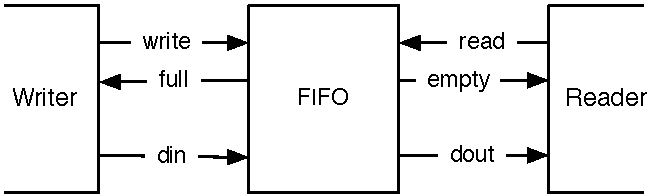
\includegraphics[scale=\scale]{figures/fifo}
  \caption{A writer, a FIFO buffer, and a reader.}
  \label{fig:fifo}
\end{figure}

A FIFO is initially empty, singled by the \code{empty} signal. Reading
from an empty FIFO is usually undefined. When data is written and never
read a FIFO will become \code{full}. Writing to a full FIFO is usually ignored
and the data lost. In other words, the signals \code{empty} and \code{full}
serve as handshake signals 

Several different implementations of a FIFO are possible: E.g., using on-chip
memory and read and write pointers or simply a chain of registers with a
tiny state machine. For small buffers (up to tens of elements) a FIFO organized
with individual registers connected into a chain of buffers is a simple
implementation with a low resource requirement.
The code of the bubble FIFO is available in the
\myref{https://github.com/schoeberl/chisel-examples}{chisel-examples}
repository.\footnote{For completeness, the Chisel book repository contains
a copy of the FIFO code as well.}

We start by defining the IO signals for the writer and the reader side.
The size of the data is configurable with \code{size}.
The write data are \code{din} and a write is signaled by \code{write}.
The signal \code{full} performs the
\myref{https://en.wikipedia.org/wiki/Flow_control_(data)}{flow control}
at the writer side.

\shortlist{code/fifo_writer_io.txt}

The reader side provides data with \code{dout} and the read is initiated
with \code{read}. The \code{empty} signal is responsible for the flow control
at the reader side.

\shortlist{code/fifo_reader_io.txt}

Listing~\ref{lst:fifo:stage} shows a single buffer. The buffer has a enqueueing port
\code{enq} of type \code{WriterIO} and a dequeueing port \code{deq} of type
\code{ReaderIO}. The state elements of the buffer is one register that holds the
data (\code{dataReg} and one state register for the simple FSM (\code{stateReg}).
The FSM has only two states: either the buffer is \code{empty} or \code{full}.
If the buffer is \code{empty}, a write will register the input data and change
to the \code{full} state.
If the buffer is \code{full}, a read will consume the data and change to the
\code{empty} state.
The IO ports \code{full} and \code{empty} represent the buffer state for
the writer and the reader.

\longlist{code/fifo_register.txt}{A single stage of the bubble FIFO.}{lst:fifo:stage}

Listing~\ref{lst:fifo} shows the complete FIFO. The complete FIFO has
the same IO interface as the individual FIFO buffers.
\code{BubbleFifo} has as parameters the \code{size} of the data
word and \code{depth} for the number of buffer stages.
We can build an \code{depth} stages bubble FIFO out of \code{depth}
\code{FifoRegister}s. We crate the stages by filling them into a Scala \code{Array}.
The Scala array has no hardware meaning, it \emph{just} provides us with
a container to have references to the created buffers.
In a Scala \code{for} loop we connect the individual buffers.
The first buffers enqueueing side is connected to the enqueueing IO of
the complete FIFO and the last buffer's dequeueing side to the
dequeueing side of the complete FIFO.

\longlist{code/fifo.txt}{A FIFO is composed of an array of FIFO bubble stages.}{lst:fifo}


\section{A Serial Port}

A serial port (also called
\myref{https://en.wikipedia.org/wiki/Universal_asynchronous_receiver-transmitter}{UART}
or \myref{https://en.wikipedia.org/wiki/RS-232}{RS-232}) is one of the easiest options
to communicate between your laptop and an FPGA board.
As the name implies, data is transmitted serially. An 8-bit byte is transmitted as follows:
one start bit (0), the 8-bit data, least significant bit first, and then one or two stop
bits (1). When no data is transmitted, the output is 1.
Figure~\ref{fig:uart:wave} shows the timing diagram of one byte transmitted.

\begin{figure}
  \centering
  \includegraphics[scale=1]{figures/uart_wave}
  \caption{One byte transmitted by a UART.}
  \label{fig:uart:wave}
\end{figure}

We design our UART in a modular way with minimal functionality
per module. We present a transmitter (TX), a receiver (RX),
a buffer, and then usage of those base components.

First, we need an interface, a port definition.
For the UART design, we use a ready/valid handshake interface,
with the direction as seen from the transmitter.
\shortlist{code/uart_channel.txt}
The convention of a ready/valid interface is that the data is transferred
when both \code{ready} and \code{valid} are asserted.

\longlist{code/uart_tx.txt}{A transmitter for a serial port.}{lst:uart:tx}

Listing~\ref{lst:uart:tx} shows a bare-bone serial transmitter (\code{Tx}).
The IO ports are the \code{txd} port, where the serial data is sent and
a \code{Channel} where the transmitter can receive the characters to serialize
and send.
To generate the correct timing, we compute a constant for by computing
the time in clock cycles for one serial bit.

We use three registers:
(1) register to shift the data (serialize them) (\code{shiftReg}),
(2) a counter to generate the correct baud rate (\code{cntReg}), and
(3) a counter for the number of bits that still need to be shifted out.
No additional state register of FSM is needed, all state is encoded in
those three registers.

Counter \code{cntReg} is continuously running (counting down to 0
and reset to the start value when 0). All action is only done when
\code{cntReg} is 0. As we build a minimal transmitter, we have only
the shift register to store the data. Therefore, the channel is only ready
when \code{cntReg} is 0 and no bits are left to shift out.

The IO port \code{txd} is directly connected to the least significant bit
of the shift register.

When there are more bits to shift out (\code{bitsReg =/= 0.U}),
we shift the bits to the right and fill with 1 from the top (the idle level
of a transmitter).
If no more bits need to be shifted out, we check if the channel contains
data (signaled with the \code{valid} port). If so, the bit string to
be shifted out is constructed with one start bit (0), the 8-bit data, and
two stop bits (1). Therefore, the bit count is set to 11.

This very minimal transmitter has no additional buffer and can
accept a new character only when the shift register is empty
and at the clock cycle when \code{cntReg} is 0.
Accepting new data only when \code{cntReg} is 0 also means
that the ready flag is also de-asserted when there would be
space in the shift register. However, we do not want to add this
``complexity'' to the transmitter but delegate it to a buffer.

\longlist{code/uart_buffer.txt}{A single-byte buffer with a ready/valid interface.}{lst:uart:buffer}
Listing~\ref{lst:uart:buffer} shows a single byte buffer, similar to
the FIFO register for the bubble FIFO. The input port is a \code{Channel}
interface, and the output is the \code{Channel} interface with
flipped directions. The buffer contains the minimal state machine
to indicate \code{empty} or \code{full}. The buffer driven handshake
signals (\code{in.ready} and \code{out.valid} depend on the state
register.

When the state is \code{empty}, and data on the input is \code{valid},
we register the data and switch to state \code{full}.
When the state is \code{full}, and the downstream receiver is
\code{ready}, the downstream data transfer happens, and we switch
back to state \code{empty}.

\longlist{code/uart_buffered_tx.txt}{A transmitter with an additional buffer.}{lst:uart:buffered:tx}
With that buffer we can extend our bare-bone transmitter.
Listing~\ref{lst:uart:buffered:tx} shows the combination of the transmitter \code{Tx}
with a single-buffer in front. This buffer now relaxes the issue that \code{Tx}
was \code{ready} only for single clock cycles. We delegated the solution of
this issue to the buffer module.
An extension of the single word buffer to a real FIFO can easily be done
and needs no change in the transmitter or the single byte buffer.

\longlist{code/uart_rx.txt}{A receiver for a serial port.}{lst:uart:rx}
Listing~\ref{lst:uart:rx} shows the code for the receiver (\code{Rx}).
A receiver is a little bit tricky, as it needs to reconstruct the timing of
the serial data. The receiver waits for the falling edge of the start bit.
From that event, the receiver waits 1.5 bit times to position itself into the middle
of bit 0. Then it shifts in the bits every bit time. You can observe these
two waiting times as \code{START\_CNT} and \code{BIT\_CNT}.
For both times, the same counter (\code{cntReg}) is used.
After 8 bits are shifted in, \code{valReg} signals an available byte

\longlist{code/uart_sender.txt}{Sending ``Hello World!" via the serial port.}{lst:uart:sender}
Listing~\ref{lst:uart:sender} shows the usage of the serial port transmitter
by sending a friendly message out. We define the message in a Scala
string (\code{msg}) and converting it to a Chisel \code{Vec} of \code{UInt}.
A Scala string is a sequence that supports the \code{map} method.
The \code{map} method takes as argument a function literal, applies this function to
each element, and builds a sequence of the functions return values.
If the function literal shall have only one argument, as it is in this case, the
argument can be represented by \code{\_}. Our function literal calls
the Chisel method \code{.U} to convert the Scala \code{Char} to a Chisel
\code{UInt}. The sequence is then passed to \code{VecInint} to construct
a Chisel \code{Vec}. We index into the vector \code{text} with the counter
\code{cntReg} to provide the individual characters to the buffered transmitter.
With each \code{ready} signal we increase the counter until the full string
is sent out. The sender keeps \code{valid} asserted until the last character
has been sent out.

\longlist{code/uart_echo.txt}{Echoing data on the serial port.}{lst:uart:echo}
Listing~\ref{lst:uart:echo} shows the usage of the receiver and the transmitter
by connecting them together. This connection generates an \code{Echo} circuit where each
received character is sent back (echoed).

\section{Exercises}

This exercise section is a little bit longer as it contains two exercises:
(1) exploring the bubble FIFO and implement a different FIFO design;
and (2) exploring the UART and extending it.
Source code for both exercises is included in the
\myref{https://github.com/schoeberl/chisel-examples}{chisel-examples} repository.

\subsection{Explore FIFO Variations}

The FIFO source also includes a tester that provokes different read and write behavior and generates a waveform in the 
\myref{https://en.wikipedia.org/wiki/Value_change_dump}{value change dump (VCD)} format.
The VCD file can be viewed with a waveform viewer, such as
\myref{http://gtkwave.sourceforge.net/}{GTKWave}.
Explore the
\myref{https://github.com/schoeberl/chisel-examples/blob/master/src/test/scala/simple/FifoTester.scala}{FifoTester} in the repository.
The repository contains a \code{Makefile} to run the examples, for the FIFO example
just type:
\begin{verbatim}
$ make fifo
\end{verbatim}
This make command will compile the FIFO, run the test, and starts GTKWave for waveform
viewing. Explore the tester and the generated waveform.

In the first cycles, the tester writes a single word. We can observe in
the waveform how that word bubbles through the FIFO, therefore the
name \emph{bubble FIFO}. This bubbling also means that the
latency of a data word through the FIFO is equal to the depth of the FIFO.

The next test fills the FIFO until it is full. A single read follows.
Notice how the empty word bubbles from the reader side of the FIFO
to the writer side. When a bubble FIFO is full, it takes
a latency of the buffer depth for a read to affect the writer side. 

The end of the test contains a loop that tries to write and read at maximum speed.
We can see the bubble FIFO running at maximum bandwidth, which is two
clock cycles per word. A buffer stage has always to toggle between empty
and full for a single word transfer.

A bubble FIFO is simple and for small buffers has a low resource requirement.
The main drawbacks of an $n$ stage bubble FIFO are: (1) maximum throughput is
one word every two clock cycles, (2) a data word has to travel $n$ clock cycles
from the writer end to the reader end, and (3) a full FIFO needs $n$ clock cycles
for the restart.

These drawbacks can be solved by a FIFO implementation with a
\myref{https://en.wikipedia.org/wiki/Circular_buffer}{circular buffer}.
The circular buffer can be implemented with a memory and
read and write pointers.
Implement a FIFO as a circular buffer with four elements, using the same
interface, and explore the different behavior with the tester.
For an initial implementation of the circular buffer use, as a shortcut,
a vector of registers (\code{Reg(Vec(4, UInt(size.W)))}).

\subsection{The UART}

For the UART example, you need an FPGA board with a serial port and
a serial port for your laptop (usually with a USB connection).
Connect the serial cable between the FPGA board and the serial port on
your laptop. Start a terminal program, e.g., Hyperterm on Windows
or \code{gtkterm} on Linux:
\begin{verbatim}
$ gtkterm &
\end{verbatim}
Configure your port to use the correct device, with a USB UART this
is often something like \code{/dev/ttyUSB0}. Set the baud rate to 115200
and no parity or flow control (handshake).
With the following command you can create the Verilog code for the UART:
\begin{verbatim}
$ make uart
\end{verbatim}
Then use your synthesize tool to synthesize the design.
The repository contains a Quartus project for the DE2-115 FPGA board.
With Quartus use the play button to synthesize the design and then configure
the FPGA.
After configuration, you should see a greeting message in the terminal.

Extend the blinking LED example with a UART and write 0 and 1 to the serial
line when the LED is off and on. Use the \code{BufferedTx}, as in the \code{Sender}
example.

With the slow output of characters (two per second), you can write the data
to the UART transmit register and can ignore the read/valid handshake.
Extend the example by writing repeated numbers 0-9 as fast as the baud rate allows.
In this case, you have to extend your state machine to poll the UART status
to check if the transmit buffer is free.

The example code contains only a single buffer for the \code{Tx}. Feel free to
add the FIFO that you have implemented to add buffering to the transmitter
and receiver. 

\chapter{Design of a Processor}

As one of the last chapters in this book, we present a medium size project:
the design, simulation, and testing of a microprocessor.
To keep this project manageable, we design a simple accumulator machine.
The processor is called \myref{https://leros-dev.github.io/}{Leros}~\cite{leros:arcs2019}
and is available in open source at \url{https://github.com/leros-dev/leros}.
We would like to mention that this is an advanced example and some computer
architecture knowledge is needed to follow the presented code examples.

Leros is designed to be simple, but still a good target for a C compiler.
The description of the instructions fits on one page, see Table~\ref{tab:leros:isa}.
In that table \code{A} represents the accumulator, \code{PC} is the program counter,
\code{i} is an immediate value (0 to 255), \code{Rn} a register
\code{n} (0 to 255), \code{o} a branch offset relative to the \code{PC},
and \code{AR} an address register for memory access.

\begin{table}
\centering
\begin{tabular}{lll}
\toprule
Opcode & Function & Description\\
\midrule
add & A = A + Rn & Add register Rn to A \\
addi & A = A + i & Add immediate value i to A \\
sub & A = A - Rn & Subtract register Rn from A \\
subi & A = A - i & Subtract immediate value i from A \\
shr & A = A $>>>$ 1 & Shift A logically right \\
load & A = Rn & Load register Rn into A \\
loadi & A = i & Load immediate value i into A \\
and & A = A and Rn & And register Rn with A \\
andi & A = A and i & And immediate value i with A \\
or & A = A or Rn & Or register Rn with A \\
ori & A = A or i & Or immediate value i with A \\
xor & A = A xor Rn & Xor register Rn with A \\
xori & A = A xor i & Xor immediate value i with A \\
loadhi & A$_{15-8}$ = i & Load immediate into second byte \\
loadh2i & A$_{23-16}$ = i  & Load immediate into third byte \\
loadh3i & A$_{31-24}$ = i & Load immediate into fourth byte \\
store & Rn = A & Store A into register Rn \\
jal & PC = A, Rn = PC + 2 & Jump to A and store return address in Rn \\
ldaddr & AR = A & Load address register AR with A \\
loadind & A = mem[AR+(i $<<$ 2)] & Load a word from memory into A \\
loadindbu & A = mem[AR+i]$_{7-0}$  &  Load a byte unsigned from memory into A\\
storeind & mem[AR+(i $<<$ 2)] = A & Store A into memory \\
storeindb & mem[AR+i]$_{7-0}$ = A & Store a byte into memory \\
br & PC = PC + o & Branch \\
brz & if A == 0 PC = PC + o & Branch if A is zero \\
brnz & if A != 0 PC = PC + o  & Branch if A is not zero \\
brp & if A $>=$ 0 PC = PC + o & Branch if A is positive \\
brn & if A $<$ 0 PC = PC + o & Branch if A is negative \\
scall & scall A & System call (simulation hook) \\
\bottomrule
\end{tabular}
\caption{Leros instruction set.}
\label{tab:leros:isa}
\end{table}

\section{Start with an ALU}

A central component of a processor is the
\myref{https://en.wikipedia.org/wiki/Arithmetic_logic_unit}{arithmetic logic unit}, or ALU for short.
Therefore, we start with the coding of the ALU and a test bench.
First, we define an \code{Enum} to represent the different operations of the ALU:

\shortlist{code/leros_types.txt}

\noindent An ALU usually has two operand inputs (call them \code{a} and \code{b}), an operation \code{op}
(or opcode) input to select the function and an output \code{y}.
Listing~\ref{lst:leros-alu} shows the ALU.

\todo{draw a nice ALU, see Wikipedia}

We first define shorter names for the three inputs. The \code{switch} statement defines the
logic for the computation of \code{res}. Therefore, it gets a default assignment of 0.
The switch statement enumerates all operations and assigns the expression accordingly.
All operations map directly to a Chisel expression.
In the end, we assign the result \code{res} to the ALU output \code{y}

\longlist{code/leros_alu.txt}{The Leros ALU.}{lst:leros-alu}

For the testing, we write the ALU function in plain Scala, as shown in Listing~\ref{lst:leros-alu-scala}.

\longlist{code/leros_alu_ref.txt}{The Leros ALU function written in Scala.}{lst:leros-alu-scala}

\noindent While this duplication of hardware written in Chisel by a Scala implementation does not
detect errors in the specification; it is at least some sanity check.
We use some corner case values as the test vector:

\shortlist{code/leros_alu_testvec.txt}

\noindent We test all functions with those values on both inputs:

\shortlist{code/leros_alu_test.txt}

\noindent Full, exhaustive testing for 32-bit arguments is not possible, which was the reason we
selected some corner cases as input values. Beside testing against corner cases, it is also useful
to test against random inputs:

\shortlist{code/leros_alu_rand.txt}

\noindent You can run the tests within the Leros project with

\begin{verbatim}
$ sbt "test:runMain leros.AluTester"
\end{verbatim}

and shall produce a success message similar to:

\begin{verbatim}
[info] [0.001] SEED 1544507337402
test Alu Success: 70567 tests passed in 70572 cycles taking
3.845715 seconds
[info] [3.825] RAN 70567 CYCLES PASSED
\end{verbatim}

\section{Decoding Instructions}

From the ALU, we work backward and implement the instruction decoder.
However, first, we define the instruction encoding in its own Scala class and
a \emph{shared} package. We want to share the encoding constants between
the hardware implementation of Leros, an assembler for Leros, and an instruction
set simulator of Leros.

\shortlist{code/leros_constants.txt}

\todo{Update code when Leros is more complete, as stuff is missing.}

\noindent For the decode component, we define a \code{Bundle} for the output,
which is later fed partially into the ALU.

\shortlist{code/leros_decode_bundle.txt}

\noindent Decode takes as input an 8-bit opcode and delivers the decoded signals
as output. Those driving signals are assigned a default value with \code{WireInit}.

\shortlist{code/leros_decode_init.txt}

\noindent The decoding itself is just a large switch statement on the part of the
instruction that represents the opcode (in Leros for most instructions the upper
8 bits.)

\shortlist{code/leros_decode.txt}

\section{Assembling Instructions}

To write programs for Leros we need an assembler. However, for the very first
test, we can hard code a few instructions, and put them into a Scala array,
which we use to initialize the instruction memory.

\shortlist{code/leros_asm_hard.txt}

\noindent However, this is a very inefficient approach to test a processor.
Writing an assembler with an expressive language like Scala is not a big project.
Therefore, we write a simple assembler for Leros, which is possible within about
100 lines of code. We define a function \code{getProgram} that calls the assembler.
For branch destinations, we need a symbol table, which we collect in a \code{Map}.
A classic assembler runs in two passes: (1) collect the values for the symbol table
and (2) assemble the program with the symbols collected in the first pass.
Therefore, we call \code{assemble} twice with a parameter to indicate which pass it is.

\shortlist{code/leros_asm_call.txt}

The \code{assemble} function starts with reading in the source
file\footnote{This function does not actually read the source file, but for this
discussion we can consider it as the reading function.}
and defining two helper functions to parse the two possible operands: (1) an
integer constant (allowing decimal or hexadecimal notation) and (2) to read
a register number.

\shortlist{code/leros_asm_start.txt}

Listing~\ref{lst:leros-asm-match} shows the core of the assembler for Leros.
A Scala \code{match} expression covers the core of the assembly function.
\todo{Some more words on the code.}



\longlist{code/leros_asm_match.txt}{The main part of the Leros assembler.}{lst:leros-asm-match}

\section{Exercise}

This exercise assignment in one of the last Chapters is in a very free form. You are at the end
of your learning tour through Chisel and ready to tackle design problems that
you find interesting.

One option is to reread the chapter and read along with all the source code in the
\myref{https://github.com/leros-dev/leros}{Leros repository}, run the test cases,
fiddle with the code by breaking it and see that tests fail.

Another option is to write your implementation of Leros.
The implementation in the repository is just one possible organization of a pipeline.
You could write a Chisel simulation version of Leros with just a single pipeline stage,
or go creasy and superpipeline Leros for the highest possible clocking frequency.

A third option is to design your processor from scratch. Maybe the demonstration of
how to build the Leros processor and the needed tools has convinced you that processor
design and implementation is no magic art, but the engineering that can be very joyful.

\chapter{Contributing to Chisel}

Chisel is an open-source project under constant development and improvement.
Therefore, you can also contribute to the project. Here we describe how to
set up your environment for Chisel library development and how to contribute
to Chisel.

\section{Setup the Development Environment}

Chisel consists of several different repositories; all hosted at
the \myref{https://github.com/freechipsproject}{freechips organization at GitHub}.

Fork the repository, which you like to contribute, into your personal GitHub account.
You can fork the repository by pressing the \code{Fork} button in the GitHub web interface.
Then from that fork, clone your fork of the repository. In our example, we change
\code{chisel3}, and the clone command for my local fork is:

\begin{verbatim}
$ git clone git@github.com:schoeberl/chisel3.git
\end{verbatim}

To compile Chisel 3 and publish as a local library execute:
\begin{verbatim}
$ cd chisel3
$ sbt compile
$ sbt publishLocal
\end{verbatim}

Watch out during the publish local command for the version string of the published
library, which contains the string \code{SNAPSHOT}.
If you use the tester and the published version is not compatible with the Chisel
SNAPSHOT, fork and clone the \myref{https://github.com/freechipsproject/chisel-testers}{chisel-tester}
repo as well and publish it locally.

To test your changes in Chisel, you probably also want to set up a Chisel project,
e.g., by forking/cloning an \myref{https://github.com/schoeberl/chisel-empty}{empty Chisel project},
renaming it, and removing the \code{.git} folder from it.

Change the \code{build.sbt} to reference the locally published version of Chisel.
Furthermore, at the time of this writing, the head of Chisel source uses Scala 2.12, but Scala
2.12 has troubles with
\myref{https://github.com/freechipsproject/chisel-template/issues/35}{anonymous bundles}.
Therefore, you need to add the following Scala option: \code{"-Xsource:2.11"}.
The \code{build.sbt} should look similar to:

\begin{verbatim}
scalaVersion := "2.12.6"

scalacOptions := Seq("-Xsource:2.11")

resolvers ++= Seq(
  Resolver.sonatypeRepo("snapshots"),
  Resolver.sonatypeRepo("releases")
)

libraryDependencies +=
  "edu.berkeley.cs" %% "chisel3" % "3.2-SNAPSHOT"
libraryDependencies +=
  "edu.berkeley.cs" %% "chisel-iotesters" % "1.3-SNAPSHOT"
\end{verbatim}

Compile your Chisel test application and take a close look if it picks up the local published
version of the Chisel library (there is also a SNAPSHOT version published, so if, e.g.,
the Scala version is different between your Chisel library and your application code,
it picks up the SNAPSHOT version from the server instead of your local published
library.)

See also \myref{https://github.com/freechipsproject/chisel3\#for-chisel-developers}{some notes
at the Chisel repo}.

\section{Testing}

When you change the Chisel library, you should run the Chisel tests.
In an \code{sbt} based project, this is usually run with:

\begin{verbatim}
$ sbt test
\end{verbatim}

Furthermore, if you add functionality to Chisel, you should also provide tests for the
new features.

\section{Contribute with a Pull Request}

In the Chisel project, no developer commits directly to the main repository.
A contribution is organized via a
\myref{https://help.github.com/articles/creating-a-pull-request-from-a-fork/}{pull request}
from a branch in a forked version of the library.
For further information, see the documentation at GitHub on
\myref{https://help.github.com/categories/collaborating-with-issues-and-pull-requests/}{collaboration with
pull requests}.
The Chisel group started to document
\myref{https://github.com/freechipsproject/chisel-lang-governance/blob/master/reviewer_guidelines.md}{contribution
guidelines}.

\section{Exercise}

Invent a new operator for the \code{UInt} type, implement it in the Chisel library,
and write some usage/test code to explore the operator. It does not need to be
a useful operator; just anything will be good, e.g., a ? operator that delivers the lefthand side
if it is different from 0 otherwise the righthand side. Sounds like a multiplexer, right?
How many lines of code did you need to add?\footnote{A quick and dirty implementation
needs just two lines of Scala code.}

As simple as this was, please be not tempted to fork the Chisel project and
add your little extensions. Changes and extension shall be coordinated with the
main developers.
This exercise was just a simple exercise to get you started.

If you are getting bold, you could pick one of the
\myref{https://github.com/freechipsproject/chisel3/issues}{open issues} and try to solve it.
Then contribute with a pull request to Chisel.
However, probably first watch the style of development in Chisel by watching the GitHub
repositories.
See how changes and pull requests are handled in the Chisel open-source project.


\chapter{Summary}
\label{sec:conclusion}

This book presented an introduction to digital design using the
hardware construction language Chisel.
We have seen several simple to medium-sized digital circuits
described in Chisel.
Chisel is embedded in Scala and therefore inherits the powerful
abstraction of Scala.
As this book is intended as an introduction, we have restricted
our examples to simple uses of Scala.
A next logical step is to learn a few basics of Scala and apply them
to your Chisel project.

I would be happy to receive feedback on the book, as I will further
improve it and will publish new editions. You can contact me at
\url{mailto:masca@dtu.dk}, or with an issue request on the GitHub
repository. I am also happily accepting pull requests
for the book repository for any fixes and improvements.

\section*{Source Access}

This book is available in open source.
The repository also contains slides for a Chisel course and
all Chisel examples: \url{https://github.com/schoeberl/chisel-book}

A collection of medium-sized examples, which most are referenced
in the book, is also available in open source. This collection
also contains projects for various popular FPGA boards:
\url{https://github.com/schoeberl/chisel-examples}

\appendix

\chapter{Chisel Projects}

Chisel is not (yet) used in many projects. Therefore, open-source Chisel code
to learn the language and the coding style is rare. Here we list several projects
we are aware of that use Chisel and are in open source.

\begin{description}

\item[\myref{https://github.com/chipsalliance/rocket-chip}{Rocket Chip}]
is a \myref{https://en.wikipedia.org/wiki/RISC-V}{RISC-V}~\cite{risc-v}
processor-complex generator that comprises the Rocket
microarchitecture and TileLink interconnect generators.  Originally developed
at UC Berkeley as the first chip-scale Chisel project~\cite{rocket:techrep}, Rocket Chip is now
commercially supported by \myref{https://www.sifive.com/}{SiFive}.
%The codebase at SiFive serves as a major test bench for Chisel and new Chisel features
%need to pass the tests at SiFive.

\item[\myref{https://github.com/ucb-bar/riscv-sodor}{Sodor}] is a collection of RISC-V
implementations intended for educational use. It contains 1, 2, 3, and 5 stages pipeline
implementations. All processors use a simple scratchpad memory shared by instruction
fetch, data access, and program loading via a debug port. Sodor is mainly intended to
be used in simulation.

\item[\myref{https://github.com/t-crest/patmos}{Patmos}] is an implementation of a
processor optimized for real-time systems~\cite{patmos:rts2018}. The Patmos repository
includes several multicore communication architectures, such as a time-predictable memory
arbiter~\cite{t-crest:memnoc}, a network-on-chip~\cite{s4nocni:arcs2019}
a shared scratchpad memory with an ownership~\cite{t-crest:ownspm}.
At the time of this writing, Patmos is still described in Chisel 2.

\item[\myref{https://github.com/pretis/flexpret}{FlexPRET}] is an implementation of a
precision timed architecture~\cite{Zimmer:EECS-2015-181}. FlexPRET implements
the RISC-V instruction set and has been updated to Chisel 3.1.

\item[\myref{https://github.com/schoeberl/lipsi}{Lipsi}] is a tiny processor intended
for utility functions on a system-on-chip~\cite{lipsi:arcs2018}. As the code base of
Lipsi is very small, it can serve as an easy starting point for processor design in Chisel.
Lipsi also showcases the productivity of Chisel/Scala. It took me 14 hours to describe the
hardware in Chisel and run it on an FPGA, write an assembler in Scala, write a
Lipsi instruction set simulator in Scala for co-simulation, and write a few test cases
in Lipsi assembler.

\item[\myref{http://www.opensocfabric.org/}{OpenSoC Fabric}] is an open-source NoC
generator written in Chisel~~\cite{OpenSoC:ispass2016}. It is intended to provide a
system-on-chip for large-scale design exploration. The NoC itself is a state-of-the-art design with wormhole routing, credits for flow control, and virtual channels.
OpenSoC Fabric is still using Chisel~2.

\item[\myref{https://github.com/bu-icsg/xfiles-dana}{RoCC}] is a neural network accelerator
that integrates with the RISC-V Rocket processor~\cite{RoCC:2015}.
RoCC supports inference and learning.

\end{description}

If you know an open-source project that uses Chisel, please drop me a note
so I can include it in a future edition of the book.

\chapter{Chisel 2}

This book covers version 3 of Chisel. Moreover, Chisel 3 is recommended for new designs.
However, there is still Chisel 2 code out in the wild, which has not yet been converted
to Chisel 3. There is documentation available on how to convert a Chisel 2 project to
Chisel 3:

\begin{itemize}
\item \myref{https://github.com/freechipsproject/chisel3/wiki/Chisel3-vs-Chisel2}{Chisel2 vs. Chisel3} and
\item \myref{https://github.com/schoeberl/chisel-examples/blob/master/TowardsChisel3.md}{Towards Chisel 3}
\end{itemize}

However, you might get involved in a project that still uses Chisel 2,
e.g., the \myref{https://github.com/t-crest/patmos}{Patmos}~\cite{patmos:rts2018} processor.
Therefore, we provide here some information on Chisel 2 coding for those who
have started with Chisel 3.

First, all documentation on Chisel 2 has been removed from the web sites
belonging to Chisel. We have rescued those PDF documents and put them
on GitHub at \url{https://github.com/schoeberl/chisel2-doc}.
You can use the Chisel 2 tutorial by switching to the Chisel 2 branch:

\begin{chisel}
$ git clone https://github.com/ucb-bar/chisel-tutorial.git
$ cd chisel-tutorial
$ git checkout chisel2
\end{chisel}

The main visible difference between Chisel 3 and 2 are the definitions of
constants, bundles for IO, wires, memories, and probably older forms of register
definitions.

Chisel 2 constructs can be used, to some extent, in a Chisel 3 project by
using the compatibility layer using as package \code{Chisel} instead of \code{chisel3}.
However, using this compatibility layer should only be used in a transition phase.
Therefore, we do not cover it here.

Here are two examples of basic components, the same that have been presented
for Chisel 3. A module containing combinational logic:

\shortlist{chisel2/src/main/scala/Logic.scala}

Note that the \code{Bundle} for the IO definition is \emph{not} wrapped into
an \code{IO()} class.  Furthermore, the direction of the different IO ports is defined
as part of the type definition, in this example as \code{INPUT} and \code{OUTPUT}
as part of \code{UInt}. The width is given as the second parameter.

\begin{minipage}{\linewidth}
The 8-bit register example in Chisel 2:

\shortlist{chisel2/src/main/scala/Register.scala}
\end{minipage}

Here you see a typical register definition with a reset value passed in as
a \code{UInt} to the named parameter \code{init}. This form is still valid in Chisel 3,
but the usage of \code{RegInit} and \code{RegNext} is recommended for new Chisel 3 designs.
Note also here the constant definition of an 8-bit wide 0 as \code{UInt(0, 8)}.

Chisel based testing C++ code and Verilog code are generated by calling \code{chiselMainTest}
and \code{chiselMain}. Both ``main'' functions take a \code{String} array for further parameters.

\shortlist{chisel2/src/main/scala/LogicTester.scala}

\shortlist{chisel2/src/main/scala/LogicHardware.scala}

A memory with sequential registered read and write ports is defined in Chisel 2 as:

\begin{chisel}
  val mem = Mem(UInt(width = 8), 256, seqRead = true)
  val rdData = mem(Reg(next = rdAddr))
  when(wrEna) {
    mem(wrAddr) := wrData
  }
\end{chisel}

\bibliographystyle{plain}
\bibliography{chisel}

\end{document}

\chapter{Headings}

\todo{Collect the headings here, but only elevate them to chapter level when some
writing is going on.}

\section{Introduction}

 * Why Chisel, what is cool about it
 * What this book is (and what not)
 * Overview of the following Chapters

\section{Basic Circuits}

 * Combinational expressions (basic gates with logic tables)
 * Combinational base circuits (chapter 8 in Culler)
 * Multiplexer (just the simple one for a start)
 * Registers

1. base functions: +, - , and or, register (with reset, with enable)


\section{Build Process and Testing}

 * A full example (blinking LED again)
 * Packages
 * Source organization (Scala)
 * Object to generate Verilog
 * Testing
 * sbt

\section{Components/Modules}

\section{Building Blocks}

 * building blocks (adder, mux, ALU, counter, memory)
 * maybe split into combinational and sequential

\section{Bundles and Vecs (better title needed)}

\section{Medium Complex Circuits (better title needed)}

3. small designs (better name): UART, FIFO, PWM, VGA, sigma delta

\section{State Machines and Data Path}

 * Covered in stuff for Dally book lecture spring 2019

\section{Memory}

 * Vec based ROM with address register
 * Vec based read/write
 * All other variations
 * Escape code in VHDL and Verilog for unsupported memories

\section{Tips and Tricks (better title needed)}

Stuff that saves a little hardware, but might not worse the less readable code

 * Counter to -1
 * Shared adder and subtractor
 * Mux with one hot encoding of select
 * little tricks: count down, add/sub


\section{Scala for Hardware Developers}

 * Simple Scala (for, if else)
 * functions for hardware generation
 * Classes and constructor
 
 \section{More Complex Testing}
 
  * As we know now sone Scala it is time to use the power of Scala for better testing

\section{Hardware Generation}

 * More advanced stuff
 * Table generation (sinus, assembler)
 
 \section{Leros}
 
  * as a more complex design
  4. full design(s): processor

\section{Chisel 2}

 * Some notes for reading Chisel 2 code
 * Update Lipsi to Chisel 3 to work on the 2 to 3 documentation
 
 \section{Chisel Projects}
 
  * Projects written in Chisel, as paper reference, some words and a URL.

\section{Appendix}

 * Basic digital circuits, e.g., transistor based inverter, half and full adder
 * With lot of links to Wikipedia



\end{document}

\subsection*{Course Abstract}

Chisel is a hardware construction language implemented as a domain specific language in Scala. Therefore, the full power of a modern programming language is available to describe hardware and, more important, hardware generators. Chisel has been developed at UC Berkeley and successfully used for several tape outs of RISC-V. Here at DTU we used Chisel in the T-CREST project and in teaching advanced computer architecture.

In this course I will give an overview of Chisel to describe circuits at the RTL, how to use the Chisel tester functionality to test and simulate digital circuits, present how to synthesize circuits for an FPGA, and present advanced functionality of Chisel for the description of circuit generators. Besides lecturing we will have lab sessions to describe small circuits and evaluate them in an FPGA.

The aim of the course is to get a basic understanding of a modern hardware description language and be able to describe simple circuits in Chisel. This course shall give a basis to explore more advanced concepts of circuit generators written in Chisel/Scala.
